\documentclass[12pt, conference, final, a4paper, onecolumn, compsoc]{IEEEtran}
% Font size onecolumn or twocolumn Use draft for notes or final for no spacing

% Includegraphics
\usepackage{graphicx}
% Coloured code
\usepackage{color}
% Code listings
\usepackage{listings} \lstset{ basicstyle=\small, showstringspaces=false,
  % commentstyle=\itshape\small\color{gray}, keywordstyle=\color{cyan}\bfseries,
  % numberstyle=\color{gray}, numbers=left, numbersep=8pt
}
% Math equations
\usepackage{amsmath}
% Paragraph spacing - very good!
\usepackage{parskip}
% Bibliography
\usepackage{natbib}
% Figure positions
\usepackage{float}
% Wrapping figures
\usepackage{wrapfig}
% Wrapping URLs
\usepackage[hyphens]{url}
% Changes size of font in captions
\usepackage{caption}
\DeclareCaptionFont{captionfontsize}{\fontsize{12}{14}\selectfont}
\captionsetup{font=captionfontsize}

% Enable numbers for some reason
\pagestyle{plain}

\begin{document}


\title{Malware Detection within Object Storage} \author{Author: Matthew
  Battagel, Supervisor: Theodoros Spyridopoulos} \markboth{Cardiff University -
  CM3203 - Final Report}{}
\maketitle{}

\subsection*{Acknowledgments - }
% Remove section from TOC
% \addtocontents{toc}{\protect\setcounter{tocdepth}{-1}}

I would like to extend my sincere gratitude to my supervisor Theo, my colleague
Harry, parents, and Lo for their unwavering support and encouragement during my
project. Their combined expertise and guidance provided were critical in the
shaping and execution of the project. I am truly thankful to all of them for
their contributions.

\bigskip

\begin{abstract}
  The rapid increase in data production has amplified the necessity for robust
  and secure data storage systems. MinIO, an open-source object storage
  platform, offers cost-effective and scalable solutions but lacks an integrated
  malware detection feature, thereby posing potential risks to user data. This
  project seeks to augment MinIO by incorporating a scalable malware detection
  system, with the goal of maintaining MinIO's performance and scalability. In
  essence, this project aspires to enhance the security features of MinIO while
  offering a valuable experience in deploying production-grade solutions within
  a microservice framework.
\end{abstract}

\pagebreak

\tableofcontents{}

\pagebreak

\section{Introduction}
\subsection{Overview}
\paragraph{}
The exponential growth of data generation has made data storage an increasingly
important aspect for both individuals and organisations alike
\citep{data-storage}. Object storage has emerged as a promising solution due to
its ability to store vast amounts of unstructured data in a cost-effective and
scalable manner \citep{object-storage-market}. Object storage improves upon
traditional storage ideas by moving lower-level functions inside of the storage
device itself to raise the level of presented abstraction to the
user \citep{object-storage}. Functions such as, space management and access
control are handled by the device while objects are accessed through a
storage interface \citep{object-storage}.

% Market and competition
One of the most widely used object storage platforms is Amazon S3, which
provides a highly scalable and reliable solution for storing data
\citep{cloud-review}. However, an open-source alternative called MinIO has
emerged as a promising contender, providing similar features to Amazon S3 while
giving customers greater control over their data \citep{minio}. MinIO is written
in Go and is available for free under the Apache License 3.0 or, for commercial
and enterprise purposes, at a reduced cost compared to Amazon S3
\citep{minio-pricing}. MinIO offers a wide range of features, including high
performance, data replication, encryption and erasure coding \citep{minio}. Most
importantly, MinIO is designed to scale out horizontally to ensure that it can
handle the demands of large-scale applications \citep{minio}.

% Scalability
With MinIO, scalability is made simple by allowing multiple types of hardware
platforms to work together in separate nodes each with their own compute and
storage within a microservice architecture \citep{minio}. This is extremely
attractive for customers who want to utilises their existing hardware without
being tied down to a specific provider. This also applies for customers looking
to migrate their data from Amazon S3 to cheaper solutions without compromising on
the high performance, reliability and scalability of the S3 platform.

% Downsides
While MinIO is a great alternative to Amazon S3, it does not offer any form of
integrated malware detection. This could deter potential customers from choosing
MinIO as a viable platform to migrate to from Amazon S3 or leave existing users
data vulnerable to malware attacks. This project aims to address this issue by
integrating a malware detection system into MinIO without negatively impacting
the scalability or performance such that MinIO is still an effective alternative
to Amazon S3.

\subsection{Motivation} % Why am I trying to add malware detection for object storage?
\paragraph{}

Due to the high amount of unstructured data expected to be both written to and read
from to the object store, and the increasing amount of malware being produced
\citep{sophos}, there are increased risks of encountering malicious files.
Therefore malware detection within object storage is crucial in modern cloud
storage scenarios. Most popular off-the-shelf object storage platforms, such as
AWS, already have integrated third-party antivirus software, such as ClamAV and
Sophos \citep{amazon-md}, to mitigate security risks. MinIO on the other hand is
vulnerable to malware attacks as it currently does not have any native antivirus
integration \citep{minio}. This forces customers who require complete virus protection to
either not use MinIO or to use potentially costly third-party software. As
antivirus scanning is inherently resource intensive, if the software is
integrated incorrectly, it could reduce the ability for the storage solution to
scale horizontally. The purpose of this project is to implement malware
detection within MinIO while being mindful to not impact the scalability or
performance of the platform.

\subsection{Project Aims} % What the project aims to achieve
\paragraph{}

The primary objective of this project is to integrate malware detection into
MinIO without compromising the platform's scalability or performance. The
solution must be able to detect malware within files uploaded to MinIO and deal
with them accordingly. The solution should also be as production-ready as
possible and offer the required features customers desire in the real-world.
This includes; the ability to configure the solution, provide both metric
collection and audit logging for monitoring, and the ability for it to scale to
meet the users demand.

From a personal standpoint, this project serves as an opportunity to enhance my
knowledge of the Go programming language and the MinIO platform. Additionally,
it aims to expand my experience in designing and implementing production-ready
solutions within a microservice environment. Lastly, this project seeks to
develop my proficiency in managing time, scope, and resources for large-scale
projects.

\section{Background}

\subsection{Signature Detection} % How does signature detection work?
\paragraph{}

Signature-Detection is a method used to detect malware within files. A signature
is a string that represents a malicious file \citep{intrusion-detect}. These
signatures come in multiple forms; including MD5 hashes, to represent whole-files
\citep{sig-detection}, byte sequences, which can be matched internally or regex
patterns, often written in YARA \citep{yara}, to allow for more fuzzy matching.
If malware were to have a different signature than the one present in the virus
database, fuzzy matchers like YARA could be used to compare more abstract
properties of the file using a set of rule \citep{yara}. These rules are reverse
engineered from known malware to include common indicators of compromise (IOC)
like text or hex strings \citep{yara-rules}.

However, signature detection is not foolproof. It is ineffective against unknown
malware or significantly modified variants of existing malware
\citep{intrusion-detect}. This requires frequent updates to the signature
database to ensure that knowledge of new malware is kept up to date. In
addition, YARA rules can be generated automatically but are often not as
effective as manually generated ones \citep{yara}.

\subsection{Malware Detection with ClamAV}
\paragraph{}

ClamAV uses the latest signature-based detection techniques to scan files
located on the disk \citep{splitscreen}. It is the most popular open-source
antivirus software and has already been optimised to use less memory and to
speed up signature matching \citep{splitscreen}. ClamAV pulls its signatures
from an online database which contains two types of signatures, MD5 whole-file
signatures and multi-part patterns \citep{string-matching}. ClamAV uses both of
these signatures in its detection process, firstly prioritising the single
sequence signatures and if no match then using the multi-part patterns
\citep{string-matching}. ClamAV has frequent updates to its signature database
to negate the disadvantages of signature detection \citep{clamav}.

\subsection{Microservices} % Best ways of implementing AV into a micro-service?
\paragraph{}

Microservices are a software development technique that structures an
application as a collection of loosely coupled services with high internal
cohesion. This allows for each service to be independently deployable into
logical business functions providing a high level of scalability and flexibility
\citep{microservice}. Cloud-native applications are often built using a
microservice architecture to take advantage of scaling for variable demand
\citep{microservice}. Developing a microservice also comes with
challenges that should be addressed, such as service discovery, load balancing,
and inter-service communication \citep{microservice}.

Microservices are often deployed using containerisation technologies,
orchestrated by tools such as Kubernetes \citep{kubernetes}. These containers
are housed within pods, the smallest and simplest unit in the Kubernetes object
model that encapsulates an application's container (or group of tightly-coupled
containers), storage resources, a unique network IP, and options that govern how
the container(s) should run \citep{k8s-struct}.

Each pod is deployed onto a node, which represents a single machine in a
Kubernetes cluster. This node could be a physical machine in a datacenter or a
virtual machine in a cloud environment \citep{k8s-struct}. Nodes host one
or multiple pods and provide the runtime environments for those pods'
containers.

For larger deployments, multiple nodes are organised into a cluster, managed by
a master node that coordinates activities across worker nodes
\citep{k8s-struct}. This setup allows a microservice architecture to
fully leverage the scaling and resiliency features offered by Kubernetes
\citep{kubernetes}.

Communication within and across these nodes, pods, and containers is a vital
aspect of a microservice architecture. Internally, containers within a pod can
communicate with each other directly, while inter-pod communication is managed
via the Kubernetes networking model \citep{k8s-network}.

Kubernetes facilitates exposure of services outside of the cluster through
methods like NodePort, LoadBalancer, Ingress, and ExternalName, each offering
different capabilities and trade-offs \citep{k8s-struct}. For instance,
NodePort opens a specific port on every node, while LoadBalancer and Ingress are
typically used in cloud environments to route incoming traffic, and ExternalName
maps a service to a DNS name \citep{k8s-struct}.

\subsection{Amazon S3 Malware Detection} % How does amazon do it?
\paragraph{}

As MinIO's largest competitor, this project draws a lot of inspiration from
Amazon S3's integrated malware detection article \citep{amazon-md}. The article
explains Amazons current approach for managing malware detection within their
service. Amazon S3 uses a combination of ClamAV and Sophos as their third-party
scanning engines due to their out-of-the-box nature \citep{amazon-md}. Amazon then gives you the
option to use either of these engines or both. The article goes on to describe the
three main interaction mechanisms that Amazon S3 uses to flag files for
scanning. Firstly, an API endpoint is provided to handle all uploads. This
forms a queue of uploads which are then scanned before entering the bucket.
Next, event-driven scanning is used keep track of all regular file uploads. The
antivirus will then scan each file after they have been written to the bucket.
Finally, retro-driven scanning is used to scan all existing files within the
bucket. The user then has the flexibility to define what types of files should
be scanned including defining time windows. This article has given some useful
methodologies of how to keep track of both incoming and previously scanned
files. Creating a system that can match these methods is important for offering
a matching level of scalability and security within MinIO.


% Talk about standard flow and two bucket flow - useful in designing

\section{Specification}

The purpose of the project specification is to guide the project towards
achieving the goals outlined in the previous section. The specification is
divided into three main categories; functional requirements, non-functional
requirements and constraints.

The MoSCoW method is employed to prioritize the projects requirements. It is a
prioritisation technique utilised in business analysis and software development
to establish a shared understanding among stakeholders regarding the
significance assigned to the delivery of each requirement
\citep{moscow-prioritization}. The acronym stands for:

\begin{itemize}
  \item Must have: Critical for the project's success and must be included in
        the final solution.
  \item Should have: Important but not absolutely necessary for the project's
        success. They should be included if possible, but the project can
        proceed without them.
  \item Could have: Desirable but not essential. They can be included if time
        and resources permit but can be left out without impacting the project's
        success.
  \item Won't have: Not necessary for the current project and will not be
        included. They may be considered for future development.
\end{itemize}

\subsection{Functional Requirements}
\paragraph{}

Functional requirements are provided in the table \ref{tab:functional-reqs}. The
requirement is given with a MoSCoW priority and a description to justify the
priority.

\begin{table}[H] \centering
  \begin{tabular}{|p{0.4\textwidth}|p{0.5\textwidth}|l|} \hline
    \textbf{Requirement} & \textbf{Description} & \textbf{Priority} \\ \hline
    Provide a way of detecting the latest uploads to the object store. & Key aspect
    of automatically dispatching scans based on upload. Must keep track of all
                                                                         uploads
                                                with no loss of data to ensure
                                                                         that
                                                                         all
                                                                         files
                                                                         get
                                                                         scanned.
                                                & Must \\ \hline Record the results of the malware
    detection within the object store. & Must provide feedback to the user
                                         informing them of the result from the
                                         scan. Relevant information must be
                                         provided such as, result and time scanned.  & Must \\ \hline Provide the ability to measure
    key performance and analysis metrics. & Metric
                      collection is very attractive for satisfying
                                            production-ready status. Also vital
                                            for viewing overall system health
                                            and proving that no data has been lost. & Must \\
    \hline Scale alongside MinIO to ensure that it does not bottleneck the
    object store at high loads. & To handle maximum throughput, the solution
                                 should scale alongside MinIO. This prevents the
                                                object store from being
                                  bottlenecked by the solution. & Must \\ \hline Provision
    for future expansion and ongoing maintenance. & Having the ability to build
                                                   on-top of the project will
                                                   increase the attractiveness
                                                   to users looking to migrate
                                                   from AWS. & Must \\ \hline
    Must be cost effective and legally viable for commercial use. & As the
                                                                    solution is
                                                                    targeted
                                                                    towards
                                                                    industry
                                                                    use, it must
                                                                    only use
                                                                    software
                                                                    that
                                                                    allows it to
                                                                    be used in
                                                                    production.
                                                                    This include
                                                                    compliance
                                                                    with
                                                                    licenses and
                                                                    regulations,
                                                                    cost-effective
                                                                    software and
                                                                    redundancy
                                                                    if an
                                                                    external
                                                                    software
                                                                    were to
                                                                    become
                                                                    unusable. &
                                                                                Must
                                                                                \\ \hline
    \hline

    % SHOULD
    Have a high level of customisability to allow for different use cases. &
                                                                            Gives flexibility to the user but is not a requirement for proof of concept. &
                                                                                                                                                          Should \\ \hline Allow for efficient and transparent debugging in the event of
    failure & Creating a robust product mitigates the priority of debugging. &
                                                                               Should \\ \hline

                                                                               % COULD
    Add more complex metrics - Histogram, Gauges, etc. & Additional metrics are
                                                        more beneficial in a production environment but unnecessary for size of project
                                                        scope. & Should \\ \hline \hline Provide the choice of multiple antivirus
    engines & Not necessary for the proof of concept as it requires too much time. &
                                                                                     Could \\ \hline Provide a warning when under ``delete'' cleanup policy. & Not
                                                                                                                                                              necessary for the proof-of-concept as it requires too much time. & Could \\
    \hline Automatically setup bucket notifications to be sent to the event queue. & Can be completed
                                                               manually with instructions instead. Removes customisability from the user if
                                                               done automatically. & Could \\ \hline Supply the MinIO policies the solution
    will use e.g. ``put'' and ``get''. & MinIO denies by default and therefore
                                         operations could fail when MinIO is not run with admin permissions. & Could \\
    \hline \hline

    % WON'T
    Prevent the downloading of files if flagged as infected. & Is
                                                              covered by cleanup policies. Would also require GUI changes. & Won't \\ \hline
    Protection from ``inside man'' attacks. & The system will be maintained by an
                                             admin. The admin could attempt to compromise the system. Protection against this
                                             is significantly harder without reducing extensibility. & Won't \\ \hline Provide
    multiple types of scanners e.g. hash or server based AV scanner. & These would
                                                                      have different workloads and requirements. Not achievable in project scope. &
                                                                                                                                                    Won't \\ \hline
  \end{tabular}
  \caption{Functional Requirements}
  \label{tab:functional-reqs}
\end{table}

\subsection{Non-Functional Requirements}
\paragraph{}

\begin{table}[H]
  \centering
  \begin{tabular}{|l|p{0.7\textwidth}|l|}
    \hline
    \textbf{Requirement} & \textbf{Description} & \textbf{Priority} \\ \hline
    Speed & The solution must be able to keep up with the rate of uploads made
            to MinIO. This can be measured by including a metric that records
            the scan time of each request which can then be used to find average
            scan time. & Must \\ \hline
    Scalability & The solution must scale to meet the demand of the incoming
                  requests. This can be done with scaling up, across or both.  & Must \\ \hline
    Availability & Over a long period of time, the solution must be able to handle all requests. This can be measured by comparing the number of requests made to the number of requests completed over a large time frame. & Must \\ \hline
    Reliability & 100\% of the files uploaded to MinIO must go through the scanning process. The recorded metrics can be used to compare MinIO uploads with the number of objects scanned. It is worth noting that checking the clean and infected results add to the total sum of scanned objects. & Must \\ \hline
    Capacity & The solution should be able to handle the maximum number of simultaneous requests that MinIO can handle. This can be measured by monitoring the amount of cache used by the solution under load. & Should \\ \hline
    Usability & Future additions, maintenance, and debugging should be as simple
                as possible. This requirement is more subjective and therefore
                an explanation of how this has been achieved will be discussed
                in the implementation section. Prolonged use of the solution
                should be enabled by recording dependency versions. & Should \\ \hline
    Security & The solution could implement the best practices for security,
               including data protection and secure communication between
               components. This is less of a priority as sensitive information
               is kept within the Kubernetes deployment and all external
               interaction is handled by MinIO's internal authentication. & Could \\ \hline
    Privacy & The solution is not directly responsible for following privacy
              laws and regulations, such as the DPA \citep{dpa}. & Won't \\ \hline
  \end{tabular}
  \caption{Non-Functional Requirements}
  \label{tab:non_functional_requirements}
\end{table}

\subsection{Constraints}
\paragraph{}

The primary constraint for this project is the strict 12-week timeline, which
significantly restricts the project scope. To overcome this constraint, careful
prioritisation of features and efficient time management for their
implementation is crucial.

Another constraint is the requirement that all external software used must be
open source, available for commercial use under a license, or require a fee.
This ensures the project's legal viability if the solution is to be employed
commercially.

Lastly, my personal knowledge and experience pose constraints on the project.
The learning curve for new technologies may extend the average time needed to
achieve milestones. Moreover, potential errors could result in unforeseen
delays. As a result, when selecting technologies, factors such as ease of use,
documentation, and community support should be considered to minimise the impact
of these constraints.

\section{Architecture}

\paragraph{}
Choosing the correct architecture for the project is critical for ensuring that
the solution is scalable, performant and maintainable. Given the specification
above, various potential architectures can be created and evaluated based my own
thoughts and from reading the background material. The best candidate design
will then be chosen based on which design satisfies the most
requirements with as little compromise as possible. Thought will also be given
to which architecture fits within the constraints of the project.

\subsubsection*{Project Naming}
\paragraph{}
Due to the defined functionality of the solution, an suitable name can be
chosen. ``Aegis'' is the name of the shield that Zeus used to protect himself in
Greek mythology and is also a noun synonymous with protection \citep{aegis}. This is
appropriate given that the solution is designed to protect the MinIO object
store from malware. Aegis will be used synonymously with the solution throughout
the rest of the report.

\subsection{Candidate Design 1 - Post-Write}
\paragraph{}

The first candidate design makes use of the performance benefits of MinIO by
allowing puts to be initially written to the bucket without being scanned. The
design then uses a event queue compatible with MinIO to keep track of all the
files that have been uploaded. The queue is then used to trigger a scan of the
file once an antivirus engine is available. The candidate design is shown in Figure
\ref{fig:postWriteArch}.

\begin{wrapfigure}{r}{0.45\textwidth}
  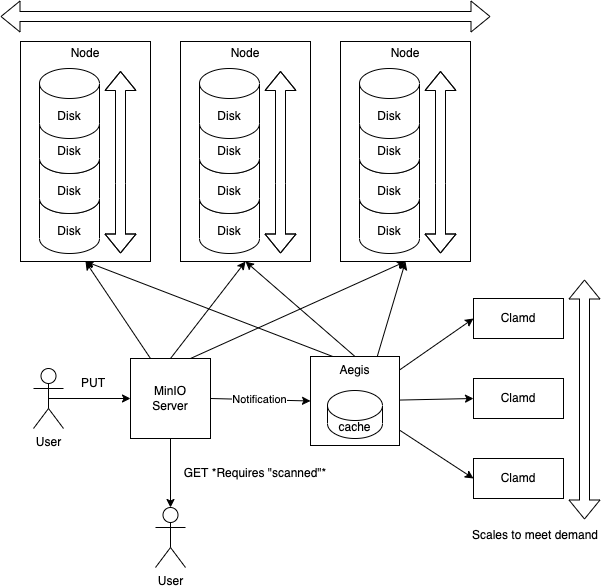
\includegraphics[scale=.4]{diagrams/post-write.png}
  \caption{Post-Write Architecture}
  \label{fig:postWriteArch}
\end{wrapfigure}

This design has many benefits over other potential implementations. Firstly, it
uses the storage provided by MinIO to store all incoming files without having to
manage a large temporary storage. This removes complexity from the
solution by not having to account for a number of failure conditions that could
occur with a high availability, production ready storage solution. For example,
the solution would not be responsible for handling partial writes, loss of data,
or data corruption. Removing this responsibility allows the solution to focus on
the core functionality of the project, the scanning of files, which is essential
for keeping the project within the time constraints.

Secondly, the design also makes use of the integrated event queue provided by
MinIO. This again removes responsibility from the solution by differing the
scalability and reliability requirements to the event queue and MinIO.

Lastly, having Aegis dispatch the files to a scalable number of antivirus
engines allows the solution to scale to meet the demands of the system. This
meets a key requirement as the solution is expected to have the capacity for a
large number of operations. This method require the use of a load balancer
to effectively distribute the load across the available antivirus scanners.

The candidate design also has a number of drawbacks. Firstly, the design still
requires a small about of cache to temporarily store the object when it is being
dispatched to the antivirus. Provisioning of this cache has to be large enough
to handle the largest file possible to be uploaded to the object store. In
reality, this cache would be provisioned even larger to allow for the temporary
storage of multiple objects while multiple scans are being performed
asynchronously. In addition, the cache needs to be large enough to ensure that
the system does not become overwhelmed by the number of objects being scanned as
the system scales. This is a minor issue as store capacity is cheap and the
provisioning of the cache easy to scale up. Additionally, a higher priority can
be given to scaling up and out antivirus engines to ensure that the smallest
number of files are being cached, while bring scanned, at any point.

The second drawback is that, for each event, Aegis makes a get request for the
object to be scanned. This effectively doubles the number of requests made to
the object store. This also means that Aegis must have the ability to get any
file expected to be scanned and therefore must have access to the whole storage
network. The impact of this drawback is mitigated as the solution is expected to
be deployed on the same network as the object store which should reduce the
latency of each request made by Aegis. However, this still leaves MinIO to
handle twice as many requests with the performance loss being noticed mainly on
more distributed storage topologies.

Thirdly, the candidate design only allows for a single Aegis instance to
dispatch all incoming objects to available scanners and antivirus engines. This
is a potential bottleneck for the system as this instance could become
overwhelmed by the number of requests it is receiving. This is a minor issue as
the dispatching of objects to scanners is not as performance intensive as other
areas of the solution, such as the actual scanning, and therefore it is not
expected to be a major bottleneck.

Lastly, any object uploaded to the store will have a certain period of time
where it remains unchecked. In this time, the user could potentially download an
unscanned object or the object could cause harm to the store before it is
detected. Although displaying warnings when downloading unscanned or infected objects is out
of scope, in an actual implementation of the solution, GUI changes would be
needed to display these warnings.

This design is similar to the event-driven architecture used by Amazon S3 \citep{amazon-md}.

\subsection{Candidate Design 2 - Upload Queue}
\paragraph{}

This candidate design created a wrapper around MinIO that the user interacts
with instead of MinIO. This means that all puts go through Aegis before being
uploaded to the object store. The candidate design is shown in Figure
\ref{fig:uploadQueueArch}.

\pagebreak

\begin{wrapfigure}{r}{0.45\textwidth}
  \centering 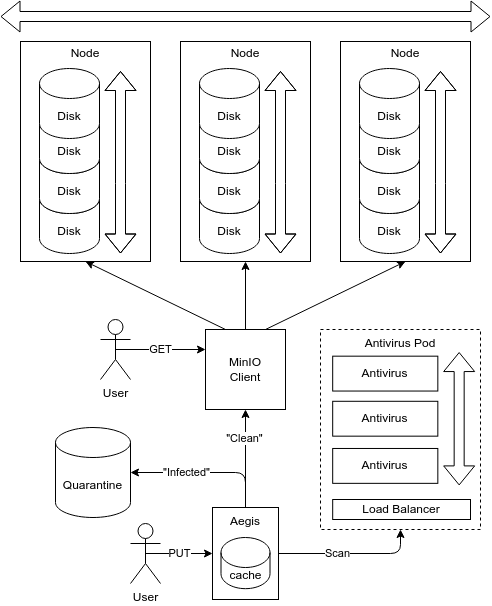
\includegraphics[scale=.4]{diagrams/upload-queue.png}
  \caption{Upload Queue Architecture}
  \label{fig:uploadQueueArch}
\end{wrapfigure}

The main benefit of this design is that the user interacts only with Aegis when
uploading files. This means that all incoming files can be stored within a
temporary storage before ever entering the object store. This offers the best
protection against malicious files as the user cannot ever download an unscanned
or infected file as it is never uploaded to the object store. Infected files can
then either be deleted or moved to a separate quarantine store for analysis.

This candidate designs main advantage also comes with a major drawback. This
design requires Aegis to handle the full throughput of all the puts to the
system. Aegis then has the full responsibility of being available to all puts
and, in a failure scenario, to handle the recovery of the system. Additionally,
the cache provisioned must be large enough to handle the largest files at
maximum throughput with extra room for unexpected delays. This negatively
affects the scope of the project by requiring the solution to prioritise
features that are already covered by MinIO. Because MinIO is dependent on Aegis
to handle the puts, MinIO must wait to be passed incoming objects sequentially
after Aegis has finished processing the previous object. Therefore, all the
performance benefits that MinIO offers are lost to time spent scanning. This
leads to users waiting longer when uploading files before they are available to
download.

This candidate design is similar to the API endpoint approach used by Amazon S3
\citep{amazon-md}.

\subsection{Candidate Design 3 - Write Interception}
\paragraph{}

Candidate Design three is very similar to the second candidate design, however,
instead of wrapping outside the MinIO service, it intercepts the writes from the
client before objects are written to the object store. With this interception,
Aegis can scan the object and decide whether to allow the object to be written
to the store or to quarantine the object. The candidate design is shown in
Figure \ref{fig:writeInterceptArch}.

\pagebreak

\begin{wrapfigure}{r}{0.4\textwidth}
  \centering 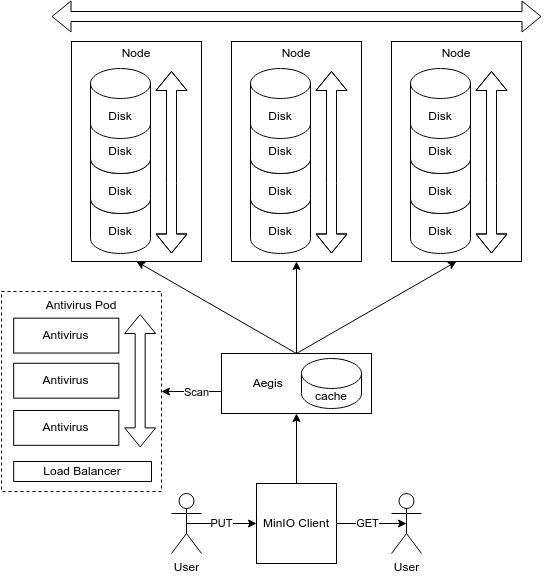
\includegraphics[scale=.4]{diagrams/write-intercept.png}
  \caption{Write Interception Architecture}
  \label{fig:writeInterceptArch}
\end{wrapfigure}

This candidate design has similar benefits as the second candidate design. It
offers the most protection against malicious files by never allowing either
unscanned or infected objects to be stored in the object store. However, it also
has similar drawbacks. This is because Aegis is still in sequence with MinIO
meaning that for optimal throughput, Aegis would need to match the performance
of MinIO.

Similar to the upload queue candidate design, this design also requires Aegis to
have a large cache to handle the largest files at maximum throughput. This cache
must also be large enough to handle the number of objects being put by MinIO
into the store. This issue cannot be mitigated without the risk of compromising
performance at increased loads.

However, this design does have an advantage over the second candidate design as
there is less responsibility placed on Aegis to be as failure tolerant. MinIO is
still directly responsible for accepting objects into the store and therefore is
still responsible for the recovery of the system in a failure scenario. This
allows the scope to focus on more related features to malware scanning.

\subsection{Candidate Design 4 - Per Node}
\paragraph{}

The final candidate design distributes Aegis onto each node in the object store.
This means that each node has a local instance of Aegis that is responsible for
scanning objects before they are written to the store. The candidate design is
shown in Figure \ref{fig:perNodeArch}.

\pagebreak

\begin{wrapfigure}{r}{0.5\textwidth}
  \centering 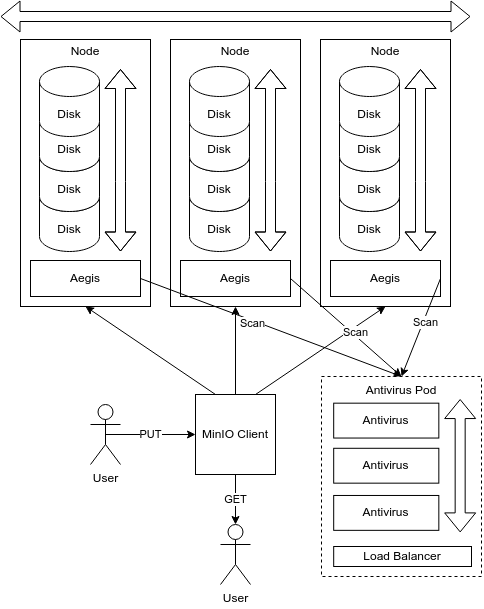
\includegraphics[scale=.4]{diagrams/per-node.png}
  \caption{Antivirus per Node Architecture}
  \label{fig:perNodeArch}
\end{wrapfigure}

This candidate design makes use of the distributed nature of MinIO to match the
demand when scaling out the system. As more nodes are added, more Aegis
instances are added to handle the increased scanning demand. This removes the
need for having a cache repository as Aegis already has access to the files that
need scanning. By removing this single point of failure, in theory, the system
only relies on the antivirus pod to be able to scale out on its own.

Independent scaling of the antivirus pod allow for efficient usage of available
hardware. A simple load based auto-scaler can be used to scale the number of
pods based on the current load. This allows for the system to scale with the
demand of the system or to reduce usage of valuable resources, such as power.
There is also the opportunity to use intelligent scaling techniques to predict
the load on the system and prematurely scale the system to meet the demand. For
example, to scale the number of pods depending on the time of day or the day of
the week.

The major drawback of this candidate design is that it replies on the ability to
scan whole files by only using data on a single node. In actual implementations,
MinIO makes use of erasure coding to add increased redundancy to the store
\citep{minio-erasure}. Erasure coding splits objects into multiple parts known
as blocks, and then calculates corresponding parity blocks. These data and
parity blocks are then distributed among all nodes in the system allowing for
on-the-fly data recovery even with the loss of multiple drives or nodes. This
means that the Aegis instance on each node only has access to the part available
on their node and therefore will not be able to reconstruct the whole file for
scanning. This makes this candidate design unsuitable for MinIO as erasure
coding is one of its key data protection features.

\subsection{Selected Candidate Design}

Given the above evaluations of each candidate design, design one best meets the
requirements and constraints of the project. It makes the most use of the
existing features that MinIO provides in order to handle failure scenarios and
to scale out. This also means that this design has less critical responsibility
and will better fit the scope constraints allowing for more time to be spent on
supplementary features, such as testing, logging, and metric collection. Because
of this, the produced solution will be closer to production-ready than the other
candidate designs.

This candidate design keeps the user in control by giving them the ability to
store unscanned files / known malware without wasting resources on a scan.
Protection can be added per bucket therefore a user could have a known malware
bucket and a clean bucket within the same object store. This allows for the
system to be more flexible and to be able to handle more use cases. Candidate
Designs two and three would not be as able to handle this use case as they both
scan all objects before they are written to the store.

The size of the cache required is smaller than all other candidate designs as it
only needs to store the objects actively being scanned. This is in opposition to
upload queue and write interception candidate designs as they have to be
prepared to handle the full demand placed on the store. This makes candidate
design one the most lightweight of all the candidate designs which should lead
to a smaller resource footprint.

In the event of an error or high demand, a backlog of requests would be stored
on the event queue enabling system to recover from a failure scenario without
losing any scan requests. This is in contrast to the other candidate designs
where the incoming requests are directly handled by Aegis and in the event of a
failure or high demand, the requests would be lost. This is an example of event
driven architecture (EDA), the asynchronous processing of events, being used to improve the reliability of the system \citep{event-driven-arch}.

\section{Implementation}

\subsection{Service Selection and Creation}
\paragraph{}

Throughout the implementation, the development of the solution followed a
waterfall approach. The project's progress was determined by milestones outlined
in the project plan Gantt chart, which can be found in the appendix at Figure
\ref{appendix:gantt}. As this is a solo project with a limited timeline, the
waterfall methodology is a better fit than an agile methodology as agile caters
more to larger teams with longer timelines where the requirements are less
concrete.

Before beginning to implement the solution, it was necessary to research,
create, configure, and understand each external service that would be used. Up
to this point, the types of services needed were identified, but the specific
services to be used had not been determined. This section will describe the
process of selecting each service and then initially configuring them to form a
bare-bones proof of concept.

\subsubsection*{Object Store - MinIO}
\paragraph{}

The object store is the only service that did not require further research or
comparison as it is already the subject of this project. However, creating and
configuring a local instance of MinIO for development was necessary. MinIO
itself is available from various sources, including Docker, Homebrew, and the
MinIO website. Homebrew, a MacOS package manager, was chosen as it is the
easiest to install and update. The MinIO documentation was then used to create a
local instance of MinIO accessible through the web client
at \url{http://localhost:9000}. This allowed for the creation of buckets,
uploading objects to the store, and familiarisation with MinIO's features. An
image of the MinIO console is available in the appendix at Figure
\ref{appendix:minio-console}.

MinIO has integrated the ability to send notifications to event queues depending
on the operation performed on the store. This makes it quick and easy to set up
a locally running instance of an event queue to read messages sent by MinIO.
MinIO offers wide support for many different event queues, such as Kafka,
Webhook, Redis, PostgreSQL, and many more.

\subsubsection*{Event Queue}
\paragraph{}

An event queue is needed to store the incoming events produced from MinIO
whenever a put event is triggered. The event queue must be able to handle a high
throughput of events and be able to scale out to meet the demand of the system
\citep{event-driven-arch}.

Kafka is a popular and well-supported event queue that is used in many different
industries \citep{event-driven-arch}. It offers many features that make it a
good choice for this project, such as high-throughput, low latency, and
open-source. Kafka is also available from both Docker and Homebrew, making it
easy to install and run locally. Most modern event queues offer similar high
throughput and low latency, but Kafka is lighter in resource usage than other
queues, such as RabbitMQ \citep{kafka-rabbitmq}. This is beneficial as it will
be easier to implement and not overuse resources when it has a simple use case.

Kafka has a dependency on Zookeeper, which is a distributed coordination service
\citep{event-driven-arch}. Zookeeper must be installed as a separate service but
is available from the same sources as Kafka. Kafka can be run in Kafka Raft mode
(KRaft), which will eventually replace Zookeeper, but as of writing KRaft, has
not been fully adopted yet \citep{kafka-raft}.

With Kafka and Zookeeper set up, the Kafka command line interface (CLI) was used
to start the service and create a topic. The MinIO documentation was then used
to configure MinIO to send all put notifications to the Kafka topic. The Kafka
CLI was used to read messages from the topic and see the messages sent by MinIO.
This demonstrated that the event queue is working and that MinIO is sending
messages to it whenever a put operation is performed. An example Kafka message
is available in the appendix under listing \ref{appendix:kafka-notif}.

\subsubsection*{Antivirus}
\paragraph{}

The antivirus chosen needed to meet a list of requirements for it to be suitable
for use in this project. Firstly, it must be able to scale with the solution in
order to keep up with the demand placed on the system. Secondly, it must have a
CLI that the program can interact with in order to scan files. Finally, it must
be free or as inexpensive as possible to make it viable for commercial use. This
narrows down the available options to a few contenders.

Sophos is a popular antivirus that is used by many businesses and is available
for free for personal use. However, it has some major downsides. It is more
costly for commercial use than ClamAV and uses more naive signature detection techniques as
stated in \citep{sophos}. This makes it less suitable for this project.

ClamAV, on the other hand, is completely free and open-source. It comes with a
scalable and multi-threaded daemon that can be accessed via CLI for
high-performance and on-demand file scanning \citep{clamav}. It is capable of
scanning many different file types, including archives and mail files. Built-in
is freshclam, a tool for automatically updating the virus database definitions.
The virus database itself is also open-source and is updated regularly by the
open source community. Although ClamAV is not the fastest or most accurate
antivirus, it offers a good starting point to building a solution with multiple
antivirus engines for higher accuracy as stated in \citep{av-comparison}. ClamAV
has a docker image and is available from Homebrew.

ClamAV was chosen for this project because it is entirely free for commercial
use, open-source, and has a CLI that can be used to scan files. It is also very
well documented and has a large community of users who regularly update and
maintain the virus database.

ClamAV comes with a daemon, clamd, that can be run in the background and can be
accessed via a CLI using clamdscan, the clamd client. A configuration file is
needed to point clamdscan to the IP address that the daemon is running. In this
case, it is running locally on port 3310. Performing the clamdscan command and
providing a file will scan the file and return the result. An example of this is
available in the appendix in listing \ref{appendix:clamd-scan}.

Aegis will be designed so that it can be easily extended to support multiple
antivirus engines aggregated together for higher accuracy \citep{av-comparison}.
Initially, only ClamAV will be implemented.

\subsubsection*{Metric Collection}
\paragraph{}

As the project is expected to be as production-ready as possible, a system for
collecting metrics is needed. This will allow the system to monitor its activity
for easier maintenance, debugging and to aid in the evaluation section of this
report. A few different options are available for metric collection, such as
Prometheus, InfluxDB, and Graphite with Prometheus being the best option as it
is open-source and the most popular metric server. It uses a pull model which
periodically scrapes metrics from a specified address and endpoint. Prometheus
then aggregates the results from the scrape and stores them in a time-series
database \citep{prom-docs}. This database can be queried through Prometheus or
exposed to another graphing service, such as Grafana.

Prometheus also has the ability to gather metrics short-term processes via a
push gateway which pushes metrics on completion instead of waiting for the
scrape period. However, this is not needed for this project as centralised
metric collectors will be used to continually aggregate and expose metrics.
Prometheus is available for download from Homebrew as well as a Docker image
available.

Prometheus is currently unusable as it is not being sent any metrics to collect.
However, the Prometheus server can still be launched, and the web interface can
be accessed on port 9090 \citep{prom-docs}. In the meantime, a configuration
file can be created, defining the address and endpoint expected to be exposing
metrics to, in this case, address \texttt{localhost:2112} and \texttt{/metrics}.

\subsubsection*{Audit Log Store}
\paragraph{}

Production-ready software should have a method to store logs for auditing and
analysis purposes. A central database can be used due to the relatively low
amount of data needing to be written and stored. The audit log's purpose is to
store information about the scans performed by the system, such as the time and
result of the scan, as well as the antivirus used. In the case that the scan
returns an infected result, the type of malware found should be recorded. This
allows the system to review previous scans, which can aid in debugging and
maintenance.

PostgreSQL is an open-source object-relational database management system
compliant with SQL standard queries \citep{postgresql}. Since the use case is
simple, SQL queries can be used to perform all actions needed when recording
audit logs shown in the PostgreSQL guide \citep{psql-guide}. PostgreSQL is also
available from both Docker and Homebrew.

At this stage, PostgreSQL is not yet storing any data. However, the PostgreSQL
server can be launched, and the database accessed via the PostgreSQL shell
prompt (psql). A database and a user for the database can be created. The
database can then be exposed to port 5432 on the localhost, making it ready for
Aegis to use.

\subsubsection*{Data Visualisation}
\paragraph{}

The final dependency that needs to be configured is a data visualisation tool.
This will not directly be implemented into the microservice but instead will be
connected to Prometheus to display the metrics collected. Grafana is a popular
open-source data visualisation tool that allows you to visualise and query the
metrics produced \citep{multi-cloud}. Grafana enables the creation of dashboards
that can display multiple relevant metrics in a single view. Data visualisation
will be an important part of this project for both the evaluation section and
for the system's ongoing maintenance.

\subsection{Aegis Module Design and Creation}
\paragraph{}

Now all of the dependencies have been downloaded, initialised and configured,
the Aegis Go module can be created. The most common language to use for
microservice based projects is GoLang. Go is a compiled language that is
statically typed and high concurrency support. This makes it a perfect fit for
this project to ensure that the system is as performant as possible. MinIO is
also written in Go should allow for easier integration. Go has certain standards
and guidelines for clean architecture that should be followed to ensure high
usability and efficiency.

Go introduces some specific language that are commonly used during the project \citep{effective-go}.
A list of common terms and their definitions are available in table
\ref{table:go-terms}.

\begin{table}[H]
  \centering
  \begin{tabular}{|l|p{0.7\textwidth}|}
    \hline
    \textbf{Go Specific Term} & \textbf{Definition} \\
    \hline
    Go keyword & Launches a function as a goroutine, which is a lightweight thread managed by the Go runtime, enabling concurrent execution. \\
    \hline
    Select    & Waits on multiple communication operations, typically used with channels, to handle different cases depending on which operation is ready. \\
    \hline
    Switch    & Multi-way branching statement that allows conditional execution of code blocks based on the evaluation of an expression or comparisons. \\
    \hline
    Goroutine & Lightweight thread managed by Go runtime, allowing concurrent execution of functions without the overhead of managing traditional threads. \\
    \hline
    Channel   & Communication mechanism between goroutines, allowing them to synchronise and share data, providing a way to safely pass data between them. \\
    \hline
    Struct    & Composite data type for creating custom structures composed of different fields, useful for grouping related data together. \\
    \hline
    Package   & Collection of related Go source files organised under a specific namespace, allowing code organisation, reuse, and dependency management. \\
    \hline
    Module    & Collection of related Go packages, providing versioning and dependency management, simplifying the process of building and sharing Go code. \\
    \hline
    Capitalised first letters & All functions, variables and types that are
                                intended to be exported outside of a package must be capitalised. \\
    \hline
    Defer & Defers the execution of a function until the surrounding function returns. \\
    \hline
  \end{tabular}
  \caption{Go Specific Terms and Their Definitions}
  \label{table:go-terms}
\end{table}

\subsubsection*{Project Structure}
\paragraph{}

In Go you should the separate the code into different packages, where each
package represents a distinct function of the system. This allows for easier
maintenance and debugging in the future. These packages are then grouped into
different directories depending on their intended scope and function. There are
three main directories that are used in GoLang projects, cmd, pkg and internal.
The cmd directory is used to store the main.go file which manages the workflow
and is the entry point of the program. The pkg directory is used to store all of
the packages that are intended to be used by external applications, in this case
our other services. The internal directory is used to store all of the packages
that are intended to be used by the application itself. This is where the
packages in the pkg directory will be consumed to perform the Aegis' core
actions as follows:

\begin{itemize}
  \item Listen for PUT events on the event queue
  \item Read the message from the event queue and extract the bucket and object
        path
  \item GET the object from the object store and store in cache
  \item Initiate a scan on the object using the antivirus software
  \item Collect the result of the scan and add tags to the object
  \item Collect metrics throughout the process
  \item Store the result of the scan in the audit log
  \item Expose metrics to Prometheus
\end{itemize}

From these requirements, the internal design of Aegis can be planned. We can
visualise this plan using various UML diagrams such as, class, sequence and flow
diagrams. Class diagrams are useful for understanding the relationships between
different classes - in this case packages - and what attributes and methods they
require \citep{class-diagrams}. It is worth noting that Go itself does not have
classes but instead uses structs which can be used to achieve the same effect.
Sequence diagrams are also valuable for understanding the timeline of the system
during the execution of a workflow \citep{uml-diagrams}. Flow diagrams are
useful for visualising the flow of processes and decisions during a workflow.
This class diagram is shown in the appendix at Figure
\ref{appendix:class-diagram} along side with a both the sequence and flow
diagram at Figures \ref{appendix:general-sequence} and
\ref{appendix:flow-diagram} respectively.

\begin{wrapfigure}{r}{0.4\textwidth}
  \centering 
\includegraphics[scale=.21]{diagrams/file-struct.png}
  \caption{Aegis' Initial File Structure}
  \label{fig:file-struct}
\end{wrapfigure}

From this diagram a file structure can be created inline with Go standards. Go
comes with a CLI tool used to initialise a new go module, which is a collection
of packages that are intended to be used together. This tool will create a go
mod file which is used to define the module and its dependencies. This tool will
also create a go sum file which is used to store the hashes of the dependencies
to ensure that the same version is used across all environments. Now go commands
can be used to install go dependencies and then download them to a local vendor
folder for use in building. Building the project is also done with the go CLI.
All binaries are stored within the build folder. The initial project structure
is shown by the Figure \ref{fig:file-struct}.

\subsubsection*{Version Control}
\paragraph{}

Considering the size of this project, version control is necessary to ensure
maintainability and the availability of a backup. Git, in combination with
GitHub, was chosen for version control due to its widespread use, familiarity,
and cost-free nature. The Git CLI was used to initialise a new repository within
the root directory of the Go module. Additionally, a \texttt{.gitignore} file
was created to prevent unnecessary files from being tracked by Git, such as, the
vendor or build folder.

To maintain usability, commits to the remote GitHub repository will be made
after each significant change to the project, accompanied by relevant commit
messages. This approach facilitates easier tracking of changes for debugging and
maintenance purposes.

\subsubsection*{Structured Logging}
\paragraph{}

Structured logging is a method of logging that allows for easier parsing of the
log messages by adding structure to the message \citep{struct-log}. This is done by adding key
value pairs containing relevant information to the log message. This enables for
easier filtering and searching of the logs. This is especially useful when using
a log aggregation tool such as, Splunk or LogRhythm \citep{struct-log}.

Go has many external modules that can handle this type of logging including Zap
by Uber. Zap is a very fast and efficient logging library that can be configured
to change the level of logging output, such as for info or debug useful for
production or development respectively \citep{zap-repo}. Zap also has the
ability to change between structured and unstructured logging depending on the
use case. Structured logging comes with the drawback of being less human
readable than unstructured logging and therefore Zap offers the ability to
change between the two \citep{zap-repo}.

As Zap is an external module, it must be added as a dependency and all code
contained in the pkg folder. A package called logger is created to encapsulate
all logging functionality. This package contains two go files, one for
interacting with the Zap and one for defining the structure of the log commands
inside of an interface. In Go, it is idiomatic to keep the interface as close to
the implementation as possible. Keeping the interface in the same package as the
implementation allows for easier mocking of the package when testing. This
package goes against this by containing the interface within the repository
because multiple packages will need to use the same interface when interacting
with them. This reduces code duplication as we don't have to define the
interface in each package that uses it, which in this case would be every
package.

\subsubsection*{Configuration}
\paragraph{}

As Aegis is a microservice, it is important that it is configurable to allow for
easy deployment to different environments. This is done by using a configuration
file in tandem with Viper, a Go module that can read in the configuration file
\citep{viper-repo}.

This configuration file contains all of the values that are likely to change
between environments. This includes values such as the endpoints, ports and
credentials of external services, logging options and database names. This
configuration file will be a dotenv file which is a key value store of
environment variables. This is beneficial as Viper has the ability automatically
override the config file with environment variables if the same key is found.
This allows for easier configuration of the application when it is built locally
or deployed in a Kubernetes cluster. This gives the user the ability to tailor
the deployment to their needs or existing implementation.

Much like the logger package, the configuration package contains two go files. A
repository file that defines the interface and a config file that contains the
Viper configuration.

Adding both the configuration and structured logging as the first packages
reduces the need for refactoring in the future. No hard coded values are needed
for initial development as all values can be stored in the configuration file
from the start.

\subsubsection*{Makefile}
\paragraph{}

A Makefile is a file that contains a set of instructions that can be run from
the command line \citep{makefile}. These instructions are used to automate processes such as
building, testing and deploying. Through the project, longer workflows will be
automated and put into the Makefile to reduce the amount of time spent on
running commands. Makefiles also simplify the usage of program by users by
encapsulating complex commands into an explicit action the user can understand.
Makefile commands can also be used by the Dockerfile when building the
application in a container.

\subsection{External Package Integration}
\paragraph{}

With the dependency services still running, the next step is to integrate them
into the Aegis application using Go. This is done by creating a new package for
each of the services within the pkg folder. Each package will contain a go file
for each of the services that will later be consumed by Aegis' internal
workflow.

One significant advantage of separating external services from internal
implementation is that it allows for a higher level of abstraction from the
services used. This abstraction provides flexibility in the use of multiple
external services that fulfill the same purpose, such as multiple antivirus
scanners. The creation of external packages allows for the use of a single
internal implementation for all of these services. This reduces the need for
extensive changes in the future, making the application more maintainable and
scalable.

\subsubsection*{MinIO}
\paragraph{}

The initial external service to be incorporated is MinIO. The MinIO package
manages interactions with the MinIO service. For this project, the required
operations include getting, putting, and removing objects, as well as getting
and putting tags. MinIO provides a Go Software Development Kit (SDK) that
already supports these operations in Go \citep{minio-go-repo}. The SDK
simplifies the complexities of making requests and offers straightforward
methods for operations such as putting and getting, as well as accessing type
definitions like tags.

Once the MinIO SDK is imported, a new MinIO client object is generated to
communicate with the MinIO service. The \texttt{CreateMinio} function accepts
essential connection parameters, such as a context, an endpoint, access and
secret keys, and an SSL usage flag, and initialises the MinIO client using the
\texttt{minio.New} function. This client object is then incorporated into a
custom \texttt{Minio} struct, along with a logger. Various methods are
implemented for the Minio struct to execute different object storage operations:

\begin{itemize}
  \item \texttt{GetObject}: Retrieves an object from a specified bucket and
        returns its data as a byte slice.
  \item \texttt{PutObject}: Takes in a byte stream and uploads it to a specified
        bucket with a specified object name.
  \item \texttt{RemoveObject}: Removes a specified object from a specified
        bucket.
  \item \texttt{GetObjectTagging}: Fetches the tags associated with an object
        and returns them as a map of key-value pairs.
  \item \texttt{PutObjectTagging}: Replaces the existing tags of an object with
        a new set of tags provided as a map of key-value pairs.
  \item \texttt{AddObjectTagging}: Adds new tags to an object by first fetching
        the existing tags, updating them with the new key-value pairs, and then
        setting the updated tags back to the object. Necessary for not
        overriding existing object tags that may exist.
\end{itemize}

All of these methods take in a context which is used in the shutdown process to
close the connection to the MinIO service. This context is passed in during the
creation of the MinIO struct so that all methods have access.

\subsubsection*{Kafka}
\paragraph{}

The next external service to be integrated is Kafka. The Kafka package will
handle the interactions with the Kafka service. For this project, the operations
needed are to consume messages from a specified topic. Kafka provides a Go
library, \textit{kafka-go}, which simplifies the consumption of messages in a Go
application \citep{kafka-go-repo}.

The package imports necessary dependencies and creates a custom
\texttt{KafkaConsumer} struct, which embeds a \texttt{kafka.Reader} object and a
logger. The \texttt{CreateKafkaConsumer} function initialises a new
\texttt{KafkaConsumer} instance by taking connection parameters such as the list
of brokers, the topic to be consumed, a group ID, and a maximum number of bytes
per message.

\begin{itemize}
  \item \texttt{ReadMessage}: Uses the Kafka library to halt until a message is
        received from the specified topic. It then decodes it using the
        \texttt{decodeMessage} function, and returns the bucket name and object
        key.
  \item \texttt{decodeMessage}: Decodes a Kafka message by unmarshalling its
        JSON payload and extracting the bucket name and object key. If the
        message event is \textit{s3:ObjectCreated:PutTagging}, it returns. This
        is required to break out of the infinite loop that is created when
        reading put events. Scanning and tagging an object will trigger another
        put event, which initiates another scan and tag. Specifically ignoring
        put tagging events prevents this feedback cycle.
\end{itemize}

During the shutdown process, the \texttt{ReadMessage} function is halted by
closing the context passed in. This closes the connection to the Kafka service
and therefore stops the reading of any new Kafka messages, leaving unprocessed
messages in the event queue.

\subsubsection*{ClamAV}
\paragraph{}

ClamAV is another external service to be integrated into the project. The
primary operation needed for this project is scanning a file and returning the
scan results. The ClamAV daemon can be interacted with through the command-line
interface (CLI) using the \texttt{clamdscan} command \citep{clamav-repo}.

Initially, a \texttt{ClamAVScanner} struct is created, embedding a logger. The
\texttt{CreateClamAV} function initialises a new \texttt{ClamAVScanner}
instance. Methods for the \texttt{ClamAVScanner} struct are implemented to
perform various file scanning operations:

\begin{itemize}
  \item \texttt{ScanFile}: Accepts a file path as an argument and scans the file
        using the built-in Go exec library to run the \texttt{clamdscan} command
        with the \texttt{--config} flag set to use a custom configuration file
        located at \texttt{clamav.conf}. The exec library enables the execution
        of external commands, providing the ability to interact with the ClamAV
        antivirus daemon. A process attribute is added, which starts the process
        in a different process group than the main execution. This approach aids
        in achieving a graceful shutdown later on, as calling a system interrupt
        terminates the entire process group \citep{process-groups}. As a result,
        \texttt{ScanFile} can continue executing after the shutdown, ensuring
        that no scans are interrupted. The method returns false if the file is
        clean, true if infected, and the type of malware detected. If any errors
        occur during the execution, it returns true (infected) along with an
        error message, ensuring that the worst-case scenario is assumed when it
        comes to security.
  \item \texttt{findVirusType}: Takes the output from the \texttt{clamdscan}
        command, extracts the virus type using regular expressions, and returns
        it as a string.
  \item \texttt{GetName}: Returns the name of the antivirus engine, in this
        case, "clamav". The name must be accessed through a method, as ClamAV
        will implement an interface that does not have access to any attributes.
\end{itemize}

This package can now implement the \texttt{Antivirus} interface given in the
internal scanner package and be used as an antivirus engines. More external
antivirus services can be created in the same way, as long as they implement the
\texttt{Antivirus} interface, if they are needed in the future.

\subsubsection*{Prometheus}
\paragraph{}

The Prometheus package is in charge of creating and managing an HTTP server that
exports metrics from Aegis. It does this by providing a plaintext response
containing the metrics in the Prometheus exposition format. The exposed endpoint
is then used by the Prometheus server to collect metrics from Aegis.

\begin{itemize}
  \item \texttt{CreatePrometheusServer}: Initialises a new Prometheus exporter
        by setting up a new HTTP server with the specified endpoint and path.
        The Prometheus handler, provided by the \texttt{promhttp.Handler()}
        function from the Prometheus Go client library, is linked to the given
        path, which serves the plaintext. Read and write timeouts for the HTTP
        server are established using constants since these values are not
        expected to be configurable.
  \item \texttt{Start}: Initiates the Prometheus server by calling the
        \texttt{ListenAndServe()} method on the HTTP server. An example of the
        generated plaintext output can be found in the appendix at listing
        \ref{appendix:example-exposed-metrics}.
  \item \texttt{Stop}: Handles the graceful shutdown of the Prometheus server by
        invoking the \texttt{Shutdown} method to close the HTTP server.
\end{itemize}

\subsubsection*{PostgreSQL}
\paragraph{}

The package imports necessary dependencies and creates a custom
\texttt{PostgresqlDB} struct, which embeds a \texttt{pgxpool.Pool} object and a
logger. The \texttt{CreatePostgresqlDB} function initialises a new
\texttt{PostgresqlDB} instance by taking connection parameters such as the user,
password, endpoint, and database name. It also returns a \texttt{CloseFunc}
function to close the connection when needed.

\begin{itemize}
  \item \texttt{CreatePostgresqlDB}: Is responsible for establishing a
        connection to the PostgreSQL database and returning a
        \texttt{PostgresqlDB} instance. The function takes in connection
        parameters such as the user, password, endpoint and database name.
        Additionally, it returns a \texttt{CloseFunc} function to facilitate a
        graceful shutdown of the connection pool when necessary. Instead of
        connecting straight to the database, the function uses a connection pool
        to manage connections. This allows multiple concurrent clients to
        perform operations on the database without having to wait for other
        clients to finish their transactions. In this case, when multiple files
        are being scanned at the same time and the results are being saved to
        the database, the connection pool ensures that a database connection is
        always available.
  \item \texttt{CreateTable}: Uses the connection pool to create a new table
        with the specified name if it does not exist. The table schema includes
        columns for ID, ObjectKey, BucketName, Result, Antivirus, Timestamp, and
        VirusType. The SQL query used to execute this operation is available in
        the appendix at listing \ref{appendix:create-table-query}.
  \item \texttt{Insert}: Uses the connection pool to insert a record into the
        specified table with values for ObjectKey, BucketName, Result,
        Antivirus, Timestamp, and VirusType. The SQL query used to insert is
        available in the appendix at listing \ref{appendix:insert-query}.
\end{itemize}

The PostgreSQL instance is provided with a context to close the connection to
the database when the application is shutting down.

\subsection{Aegis' Internal Workflow}
\paragraph{}
The internal workflow is the inner packages that make up the Aegis microservice.
Previously, the packages created were for interacting with external services but
now those services need to be utilised. The following packages are split up into
logical processed for handling different parts of the workflow. A breakdown of
these internal packages can be found in the appendix in Figures
\ref{appendix:class-diagram}, \ref{appendix:general-sequence} and \ref{appendix:flow-diagram}.

\subsubsection*{Metrics and Collectors}
\paragraph{}

The internal metrics collection comprises two primary components: the metric
manager and various metric collectors specific to each package. The metric
manager is responsible for managing interactions with Prometheus, which includes
executing the \texttt{Start} and \texttt{Stop} methods for handling the starting
and graceful shutdown of Prometheus respectively.

Each package contains a metric collector in a file named \texttt{metrics.go}.
These collectors define the available metrics that can be collected and exported
by the respective packages. The \texttt{promauto} library facilitates the
creation of a global registry when the metric manager is initialised. This
registry is accessed by all metric collectors to record the metrics they collect
and is also utilised by the Prometheus exporter for publishing these metrics.

\subsubsection*{Object}
\paragraph{}

The object package presents the \texttt{Object} struct as the internal
representation of an object within the object store. It includes all methods and
attributes related to an object, such as the object key (the path of the object
within a bucket) and bucket name.
Operations involving an object are performed within the object instance itself.

Since the object represents a concrete entity, there is no need for an interface
when using it. This design choice allows the object to have attributes that can
be accessed directly, without the need for getter functions.

The \texttt{CreateObject} function enables the creation of a new \texttt{Object}
instance, given a specified object key and bucket name.

The \texttt{SetCachePath} method defines the cache path for an object by
concatenating the cache path, bucket name, and object key, separated by slashes.
This method is called when an update to the cache path is needed.

The \texttt{SaveByteStreamToFile} method stores an object's byte stream in a
file. First, it checks if the path attribute is empty since, by default, no path
is provided. It returns an error if this is the case, as other types of scanners
may not always require this information to perform a scan. Next, it ensures that
the file's parent directory exists, creating it if necessary. Lastly, the method
writes the byte stream to the file using Go's built-in IO writer.

The \texttt{RemoveFileFromCache} method is responsible for deleting an object
file from the cache. It tries to remove the file specified by the object's path
attribute. If the removal is unsuccessful, it logs an error message and returns
the error.

\subsubsection*{Events Manager}
\paragraph{}
The events package includes the event manager, which is responsible for reading
messages from the event queue and forwarding scan requests to the scanner. The
\texttt{Kafka} interface provides methods for reading messages from the Kafka
queue and closing the connection. The \texttt{EventsManager} struct consists of
four fields: a \texttt{logger}, a \texttt{kafka} instance for interacting with
Kafka, a \texttt{scanChan} channel to forward scan requests and an
\texttt{eventsCollector} for gathering metrics.

The \texttt{CreateEventsManager} function creates a new \texttt{EventsManager}
instance, accepting the necessary arguments. The \texttt{Start} method of the
\texttt{EventsManager} takes in a context and then enters a loop that uses a
switch statement to first check if the context has been canceled. If it has, it
closes the \texttt{scanChan} channel, closes the Kafka connection and returns.
Otherwise, it invokes the \texttt{ReadMessage} method of the \texttt{kafka}
instance to read a message from the Kafka queue. Upon confirming that there is
no error and the message is not nil, it increments the \texttt{eventsCollector}
counter and creates a new \texttt{object.Object} instance with the received
bucket name and object key. It then forwards the object to the \texttt{scanChan}
channel for scanning.

Since the event manager runs within a goroutine, if an error occurs, it sends
the error to the provided \texttt{errChan} channel.

\subsubsection*{Object Store}
\paragraph{}
In the object store package, several structs and interfaces are defined to
handle object storage operations. The \texttt{Minio} interface contains the
abstract object store operations, such as; get, put and remove objects, as well
as get and put object tags. These are also reflected by the
\texttt{ObjectStoreCollector} in the form of metric counters that track the
number of each operation performed.

Once the object store is created by the \texttt{CreateObjectStore} function, it
can be used by the rest of the application to perform object storage operations.
In addition to the standard object storage operations, two more operations are
added to the object store: \texttt{MoveObject} and \texttt{AddObjectTagging}.
These both combine multiple standard operations into one as follows:

\begin{itemize}
  \item \texttt{MoveObject}: Retrieves an object from the source bucket, puts it
        into the destination bucket, and removes it from the source bucket.
  \item \texttt{AddObjectTagging}: Retrieves the object tags from the source
        bucket, adds the new tags to the existing ones, and puts the combined
        object tags onto the object.
\end{itemize}

\subsubsection*{Object Scanner}
\paragraph{}
The scanner package provides the functionality for multiple workflows when it
comes to scanning an object. In this instance, an object scanner refers to
process of downloading the object from the object store, performing a scan with
its antivirus engines, and then passing the result to the cleaner which will
execute the cleanup policy. Having the ability to use multiple types of scanners
allows for flexibility in the system as in the future, the workflow for scanning
an object might change. For example, if one of the antivirus engines could
require the hash of the file. In this case, another scanner called
\texttt{HashScanner} could be created to handle this alternate workflow. For
this project, the \texttt{ObjectScanner} will be the only type of scanner
implemented.

The \texttt{CreateObjectScanner} function creates a new \texttt{ObjectScanner}
instance with the following arguments:

\medskip
\begin{itemize}
  \item \texttt{logger}: A logger instance for logging messages.
  \item \texttt{objectStore}: An object store instance for downloading objects.
  \item \texttt{antiviruses}: An array of antivirus instances for scanning
        objects.
  \item \texttt{cleaner}: A cleaner instance for cleaning up objects.
  \item \texttt{auditLogger}: An audit logger instance for logging scan results.
  \item \texttt{scanCollector}: A scan collector instance for collecting
        metrics.
  \item Various configuration values, such as, \texttt{removeAfterScan},
        \texttt{datetimeFormat}, and \texttt{cachePath}.
\end{itemize}

All instances passed to the \texttt{CreateObjectScanner} function are interfaced
to both allow for future mocking and to allow for other abstract implementations
of the interfaces. Namely, the \texttt{Antivirus} interface is implemented by
the external antivirus engines.

The \texttt{ScanObject} method handles the workflow for downloading and scanning
an object. It takes in an \texttt{object.Object} instance, which it fetches from
the object store, and an \texttt{errChan} for returning errors. It then sets the
object cache path by calling \texttt{SetCachePath} on the object. With this set,
the scanner can perform a \texttt{GetObject} on the object store to retrieve the
byte stream of the object and call \texttt{SaveByteStreamToCache} with the byte
stream to save it to the cache.

The scanner can now perform a scan on the object by calling \texttt{Scan}, with
the cache location, on every antivirus engine. If any of the antivirus engines
detect the object as infected, then using the assume the worst mentality, the
file is deemed infected. The object is then passed to the cleaner to execute the
cleanup policy. During this execution various metrics are being collected by the
\texttt{scanCollector} about the scan, such as, the number of clean or infected
files, total files scanned and total errors encountered. In addition, audit logs
are also generated by the \texttt{auditLogger} for each scan by each antivirus
recording the object key, bucket name, antivirus name, scan result, timestamp
and if infected, the virus type.

After performing the scan and dealing with the results, if the
\texttt{removeAfterScan} flag is set to true, the object is removed from the
cache after scanning.

The \texttt{ObjectScanner} is will be run within a goroutine, if an error is
encountered during the scan, it will be sent to the provided \texttt{errChan}.

\subsubsection*{Cleanup Policies}
\paragraph{}

As mentioned in the previous section, the \texttt{ObjectScanner} passes the
object to the cleaner to execute the cleanup policy. The cleaner package defines
how to react given a clean or infected result from the antivirus engines.
Multiple policies are available in the \texttt{config.env} file to give the user
flexibility in how they want to deal with infected objects. These policies
include:

\begin{itemize}
  \item \texttt{Tag}: Adds a tag to the object in the object store based on the
        scan result.
  \item \texttt{Remove}: Removes the object from the object store if it is
        deemed infected.
  \item \texttt{Quarantine}: Moves the object to a quarantine bucket if it is
        deemed infected.
\end{itemize}

In \texttt{CreateCleaner} function, a new \texttt{Cleaner} instance is created
with a logger, object store, metrics and audit loggers, and various
configuration parameters such as the cleanup policy and quarantine bucket.

The \texttt{Cleanup} method is called by the \texttt{ObjectScanner} where is
passes the object after it has been scanned. This method uses a switch
statement, shown in Figure \ref{fig:cleaner-switch}, to determine which policy
to implement and executes the appropriate cleanup method. If no policy is
specified, the switch statement has a default case. In the case that a user
wants only the audit log, only a logger message will be provided. However, when
a cleanup policy is given, the corresponding cleanup method is called. Each of
these use the object store and object store to perform the cleanup.

\begin{figure}[H]
\begin{lstlisting}[language=Go]
      switch c.cleanupPolicy {
      case "tag":
        err = c.TagInfected(object, result, scanTime)
      case "remove":
        err = c.RemoveInfected(object, result, scanTime)
      case "quarantine":
        err = c.QuarantineInfected(object, result, scanTime)
      default:
        c.logger.Warnln("No cleanup policy found")
      }
\end{lstlisting}
  \caption{Cleanup policy switch statement}
  \label{fig:cleaner-switch}
\end{figure}

\subsubsection*{Dispatcher}
\paragraph{}

The \texttt{dispatcher} package is responsible for managing the scanning of
objects using multiple scanners concurrently. It defines a \texttt{Scanner}
interface with a single method, \texttt{ScanObject}, that will be implemented by
one of the available scanners. The \texttt{Dispatcher} struct contains three
fields: a \texttt{logger} for logging messages, a \texttt{scanChan} channel for
receiving object scan requests, with a \texttt{scanners} slice to hold the
available scanners.

The \texttt{CreateDispatcher} initialises a new \texttt{Dispatcher} instance
with the required fields. The \texttt{Start} method enters into a loop where it
ranges over the \texttt{scanChan} channel. If the channel is empty, the loop
will block until a new object is sent through the channel. If the channel has an
object, the dispatcher will spawn a new goroutine to handle the scan. However,
if the channel is closed, the loop will continue to process the remaining
objects in the channel and then exit \citep{go-channel-ranges}. This is because
when channels are closed, no more values can be sent to them, but the values
that have already been sent can still be received \citep{go-closing-channels}.
This is shown in the provided dispatcher loop code in Figure
\ref{fig:dispatcher-loop}.

\begin{figure}[H]
\begin{lstlisting}[language=Go]
  func (d *Dispatcher) Start(errChan chan error, done chan struct{}) {
    var wg sync.WaitGroup

    for request := range d.scanChan {
      for _, scanner := range d.scanners {
        wg.Add(1)
        go func(req *object.Object, sc Scanner) {
          defer wg.Done()
          sc.ScanObject(req, errChan)
        }(request, scanner)
      }
    }
    wg.Wait()
    done <- struct{}{} //Send empty done message
  }
\end{lstlisting}
  \caption{Dispatcher loop}
  \label{fig:dispatcher-loop}
\end{figure}

When the program receives a termination signal, there should be no loss of
information about incoming scan requests. This is a security risk as it could
lead to objects not being scanned. To prevent this, the dispatcher uses a
\texttt{sync.WaitGroup} to wait for all goroutines to finish before exiting the
program. This is done by calling \texttt{wg.Add(1)} before starting a new
anonymous goroutine to increment an active goroutine counter, and using
\texttt{defer wg.Done()} when the goroutine has finished to decrement the
counter. The \texttt{wg.Wait()} call will block until the counter is zero,
meaning all goroutines will have finishes processing \citep{go-waitgroups}. This
ensures that all scans that are currently being processed since
\texttt{scanChan} was close will be completed before the program exits.

\subsubsection*{Main}
\paragraph{}


The main package orchestrates the top-level workflow that Aegis executes
throughout its operation. The entry point of the program is the \texttt{main}
function, which performs one task - calling the \texttt{run} function and
exiting the program based on its return value. This design choice enhances
extensibility and testability since alternate workflows can be implemented while
maintaining a single entry point. Furthermore, the \texttt{run} function can be
tested without running the entire program \citep{go-tiny-abstraction}. The
\texttt{run} function serves as a abstraction from \texttt{main}, as it
encompasses Aegis' main workflow.

The \texttt{run} function is divided into three distinct sections:
Initialisation and configuration, the main loop, and cleanup. The initialisation
and configuration section is responsible for initialising all the components
Aegis requires and configuring them with the values provided by the
configuration package.

\medskip
\begin{itemize}
  \item The configuration is loaded from \texttt{config.env}, and the logger is
        created. An initial context is also created and passed to everything hat
        requires it, apart from the event system.
  \item The metric manager and various metric collectors are created, with the
        metric manager taking in the Prometheus exporter.
  \item The audit logger is implemented by the PostgreSQL database.
  \item The object store is implemented by the Minio client.
  \item The event system is implemented by the Kafka consumer with the
        \texttt{scanChan} passed in as well.
  \item The scanning workflow is created. This includes creating the antivirus
        engines, in this case ClamAV, creating the cleaner with the configured
        policy and passing both of them to the scanners, namely the object
        scanner. The scanners are then passed to the dispatcher alongside the
        \texttt{scanChan}.
\end{itemize}
\bigskip

% ---- Main loop -----

The main loop is the continuous execution of the goroutines that handle Aegis'
asynchronous operations. These are the event manager, dispatcher, and metric
manager. The goroutines are started using the \texttt{go} keyword, which spawns
new goroutine to execute the functions in a separate thread. An additional
context is created and parsed into the \texttt{Start} method of the
\texttt{eventManager}. Multiple channels are then created to handle errors,
shutdown command, and the shutdown complete with \texttt{errChan},
\texttt{shutdownChan} and \texttt{done} respectively. The \texttt{Start} methods
of the \texttt{eventManager}, \texttt{dispatcher} and \texttt{metricManager} are
called to begin the main workflow of the program. An error channel
(\texttt{errChan}) is created to handle errors generated by the event manager
and metric manager goroutines.

% ---- Shutdown -----

Finally, the shutdown section ensures a smooth termination when the program
receives an interrupt signal or encounters errors from the goroutines. The
shutdown sequence is vital as it allows Aegis to maintain the progress of
processed objects when receiving messages, enabling it to resume scanning
objects from where it left off upon restart. The shutdown sequence unfolds as
follows:

When an interrupt signal or an error from any goroutine is received, Aegis
starts its graceful shutdown sequence. A select statement is used to wait for a
message from either the \texttt{errChan} or \texttt{shutdownChan} channels. If
any of these channels receive a message, a message or error is logged, and the
shutdown sequence begins by canceling the context passed to the event manager.
This action halts the event manager from consuming messages from the Kafka
consumer and subsequently closes the \texttt{scanChan} channel. As a result,
incoming notifications remain in the Kafka queue and can be consumed by Aegis
upon restart leading to no scans lost.

The code then waits for the \texttt{done} channel to send a message, signaling
that the goroutines have completed processing the remaining objects in the
\texttt{scanChan} channel. Once this process is finished, the program stops the
Prometheus metric exporter and exits with a status code of 0, indicating a
successful operation. To better indicate the graceful shutdown process, a
sequence diagram is available in the appendix at Figure
\ref{appendix:shutdown-sequence}.

\subsection{Testing}

\subsubsection*{Unit Tests}
\paragraph{}

Unit testing is an essential aspect of software development that focuses on
testing individual units or components of a software application. The objective
of unit testing is to ensure that each component functions correctly in
isolation, thus improving the overall quality and reliability of the software.

In this project, unit tests were developed for each internal package, ensuring
that the core functionality of each package was thoroughly tested. Unit tests
were created using the built-in \texttt{testing} library. This package allows
for the easy creation and execution of test cases, as well as the measurement of
code coverage.

To facilitate the process of unit testing and ensure that the focus remains on
the functionality of the components under test, the mocking technique was
employed using the Mockery framework \citep{mockery}. This approach allows for the isolation of
individual components by replacing dependencies with mock implementations.

\subsubsection*{Mocking}
\paragraph{}

Mocking is a technique employed in unit testing to replace dependencies that
packages rely on for their functionality. This allows for the testing of
individual packages in isolation, minimising the impact of potential errors from
external sources and ensuring that tests focus solely on the functionality of
the component being tested.

A mocking framework called Mockery is utilised for this purpose. Mockery is a
tool that generates mocks implementing each interface within a package
\citep{go-tools}. It offers the ability to override methods, enabling the mock
to return a predetermined output for specific inputs. This capability can also
be extended to accommodate any input of a specific type.

To generate the mocks, mockery has a configuration file in which defines where
the mock files are created. I opted to create the mocks in the same package as
the interface to avoid any import conflicts. Creation of the mocks can be done
by the corresponding makefile command.

\subsubsection*{Code Coverage}
\paragraph{}

The command \texttt{go test} is used to run tests, which outputs the results of
all unit tests and the code coverage for the package. Code coverage is computed
as the ratio of the number of lines of code executed to the total number of
lines of code in the package, as illustrated in Equation \ref{eq:code_coverage}.
Code coverage serves as a valuable metric for assessing the thoroughness of
package testing.

\begin{equation} \text{Code Coverage Percentage} = \frac{\text{Number of lines
      of code executed}}{\text{Total Number of lines of code in an
      application}} \times 100
  \label{eq:code_coverage}
\end{equation}

By combining unit tests and mocking techniques, thorough testing of each
component's functionality was possible. Unit tests were continually updated and
refined throughout the development process, contributing to the overall quality
and reliability of the solution.

\subsection{Kubernetes Deployment}
\paragraph{}

To turn the solution into a microservice, a process is required to turn Aegis
into a self-contained business unit. This process is called containerisation and
is achieved by packaging the application and its dependencies into a single
container image. This image can then be deployed to a container orchestration
system such as Kubernetes.

\subsubsection*{Kubernetes}
\paragraph{}
Kubernetes (K8s) is an open-source container orchestration system
for automating deployment, scaling, and management of containerised applications
\citep{k8s-docs}. It groups containers into logical units called "pods" and
manages their lifecycle, networking, and storage. Kubernetes enables the scaling
of applications using multiple decentralised nodes controlled by internal and
horizontal load balancers. Kubernetes supplies a CLI tool called
\texttt{kubectl} for interacting and managing Kubernetes clusters.

\subsubsection*{Docker}
\paragraph{}
Docker is a platform for developing, shipping, and running
applications in containers \citep{docker}. Containers are lightweight, portable,
and provide a consistent environment for applications, simplifying deployment
and scaling. Docker allows developers to build and package applications and
their dependencies into containers that can run on any system with Docker
installed. These smaller, self-contained business units can be networked
together to form a microservice architecture.

\subsubsection*{K3d}
\paragraph{}
K3d is a lightweight Kubernetes distribution designed for local
development and testing \citep{k3d}. It runs Kubernetes clusters inside of Docker
containers, making it easy to create, delete, and manage clusters using the
provided CLI. K3d provides a convenient way to test Kubernetes deployments and
configurations before deploying them to a production environment. K3d uses a
configuration file called \texttt{k3d.yaml} to define the cluster's
configuration, including creating a registry for storing Docker images, exposing
ports, and mounting volumes \citep{k3d-conf}. The configuration file is
available in the Figure \ref{fig:expose-services}.

Registries are used to store Docker images that will be available for Kubernetes
to use. In this case, I create a local registry using K3d which I can then later
upload the Aegis Docker image to using the k3d CLI.

\subsubsection*{Aegis Containerisation}
\paragraph{}
For the Aegis solution to be deployed on Kubernetes, it needs to be
containerised using Docker. A Dockerfile is used to describe the steps required
to build the Docker image \citep{dockerfile} \citep{dockerfile-micro}. It contains 2 major sections.
Firstly, for building the Aegis application, it defines the base docker image, in this
case \texttt{golang:1.19}, and the instructions to compile the application. These
instructions include copying the source code to the container along with any
configuration files, such as the \texttt{config.env} and \texttt{clamd.conf} and
building the application using the makefile command.

The second stage is for the execution of the program. This stage downloads the
\texttt{clamdscan} dependency, copies over the config files and the binary from
the previous stage and then runs the application. This separation is beneficial
because after the binary is built, the source code can be deleted which reduces
the size of the image, therefore saving resource demand. Once the Docker image
is built, it can be uploaded to the local container registry, ready for use by
Kubernetes.

Kubernetes uses CrashLoopBackOff to restart containers that have crashed \citep{k8s-docs}. Each
time the pod crashes, the time between restarts increases. This is beneficial
because if Aegis launches before all of its dependencies are online, it will
enter a CrashLoopBackOff until the dependencies are online.

\subsubsection*{Helm}
\paragraph{}
Helm is a package manager for Kubernetes that simplifies the deployment and
management of applications on a Kubernetes cluster \citep{helm}. It uses
"charts" as templates for Kubernetes resources allowing for easy configuration,
versioning, and sharing of applications. Helm charts define the application's
networking, services, and dependencies, making it easy to deploy and maintain
applications in a Kubernetes environment.

Helm can be used to streamline the installation and management of all the
dependencies required for the solution. This approach saves time compared to
manually installing and configuring each dependency, as described in the
``Service Selection and Creation'' section. Each of these dependencies has its
own Helm chart, which can be found using the online Helm chart repository
Artifact Hub \citep{artifact-hub}. Artifact Hub stores the Helm charts that can
be installed and managed using Helm, along with documentation on how to
configure them.

\subsubsection*{Service Configuration}
\paragraph{}

Using this documentation, environment variables can be configured for each
deployment. Within the Helm chart, a \texttt{values.yaml} file holds the default
values for these variables, which will be passed into several template files.
These template files are used in Kubernetes to generate the appropriate
configuration settings for each deployment. By customising the
\texttt{values.yaml} file, you can tailor the deployments to suit the specific
requirements of your environment. As we have already allowed the overriding of
variables in Aegis by using environment variables, this means that configuring
the solution to work within Kubernetes is an easy task. In Figure
\ref{fig:override-env-vars}, these environment variables are overridden to
configure Aegis, in the \texttt{env:} key and all other services in their
corresponding fields.

\begin{figure}[H]
\begin{lstlisting}
  env:
    MINIO_ENDPOINT: aegis-minio.default.svc.cluster.local:9000
    KAFKA_BROKERS: "aegis-kafka.default.svc.cluster.local:9092"
    PROMETHEUS_ENDPOINT: 0.0.0.0:2112
    PROMETHEUS_PATH: /metrics
    POSTGRESQL_ENDPOINT: aegis-postgresql.default.svc.cluster.local:5432

  minio:
    auth:
      rootUser: minioadmin
      rootPassword: minioadmin

  postgresql:
    auth:
      enablePostgresUser: true
      postgresPassword: postgres
      database: aegis_antivirus

  kafka:
    auth:
      clientProtocol: plaintext
    provisioning:
      topics:
        - minio-put-events

  clamav:
    service:
      milter:
        enabled: false
\end{lstlisting}
  \caption{Overriding Environment Variables}
  \label{fig:override-env-vars}
\end{figure}

\subsubsection*{Internal Communication}
\paragraph{}

In Kubernetes, service endpoints are represented by DNS names that are
automatically generated upon service creation. These DNS names resolve to the
corresponding service's ClusterIP and remain stable throughout the service's
lifecycle. To enable communication between services, these DNS names can be used
as cluster internal addresses instead of the localhost address.

Utilising DNS names instead of ClusterIPs offers several advantages, including
the abstraction of the ClusterIP. This abstraction allows Kubernetes to change
the ClusterIP without requiring any reconfiguration of the deployment to locate
the updated IP. This is viewable in the \texttt{env:} field of Figure
\ref{fig:override-env-vars} where new internal addresses are used to configure the
services to communicate with each other within the cluster.

\subsubsection*{Exposing Services}
\paragraph{}

ClusterIP services are only accessible within the node, so to access the
services outside of the cluster, say to upload files to MinIO, a different type
of service must be used \citep{kube-svc}.

NodePort services expose the service on a static port on every node. NodePort
has ports available in the range 30000-32767. NodePort can be used with all TCP
or UDP traffic and therefore fits the purposes of all three services that need
to be exposed; the MinIO console, Prometheus metric server and PostgreSQL audit
log database. The main drawback with NodePort is that it offers no load
balancing customisation between nodes and by default round-robins traffic. This
is not ideal for a multi-node production environment but is less important as
the solution is deployed on a single node. A diagram of how NodePort
is used can be found in Figure \ref{fig:nodeport}.

\begin{figure}[H]
  \centering 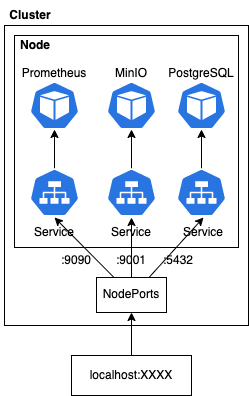
\includegraphics[scale=0.5]{diagrams/nodeport.png}
  \caption{NodePort Diagram}
  \label{fig:nodeport}
\end{figure}

The alternative to NodePort is LoadBalancer, which uses ClusterIP and NodePort
services in combination to balance traffic to all nodes in the cluster.
LoadBalancer can be configured with various algorithms to better route traffic
based on load. As this is a single node cluster, there is no need to create a
load balancer between them, so NodePort is sufficient. This can be changed in
the Helm chart if need in the future.

Below is the \texttt{k3d-conf.yaml} file that configures the NodePort services
for MinIO, Prometheus and PostgreSQL.

\begin{figure}[H]
\begin{lstlisting}
  registries:
    create:
      name: registry.localhost
      host: "0.0.0.0"
      hostPort: "12345"
  ports:
    # Expose MinIO
    - port: 9001:30001
      nodeFilters:
        - server:0
    # Expose Prometheus
    - port: 9090:30090
      nodeFilters:
        - server:0
    # Expose Postgresql
    - port: 5432:30080
      nodeFilters:
        - server:0
\end{lstlisting}
  \caption{Exposing of Services}
  \label{fig:expose-services}
\end{figure}

In the appendix is an output log displaying all services, pods and cronjobs
from the command \texttt{kubectl get all} available in the Listing \ref{appendix:kube-get-all}.

\subsubsection*{Connecting Prometheus Metrics}
% When prometheus needs to connect to aegis How to connect to postgresql and
% prometheus
\paragraph{}
The Prometheus deployment must be configured to know where to scrape metrics
from. This can be done by adding annotations to the deployment, which can be
seen in Figure \ref{fig:prometheus-annotations}. These annotations tell the
Prometheus deployment to scrape metrics from the Aegis service on the port 2112.

\begin{figure}[H]
\begin{lstlisting}
    podAnnotations:
      prometheus.io/scrape: "true"
      prometheus.io/path: /metrics
      prometheus.io/port: "2112"
\end{lstlisting}
  \caption{Adding Annotation for Prometheus}
  \label{fig:prometheus-annotations}
\end{figure}

\section{Results and Evaluation}
% Evaluate against specification Compare to MinIO Find figures like average scan

\subsubsection*{Virus Database Updates}
% When prometheus needs to connect to aegis How to connect to postgresql and
% prometheus
\paragraph{}
On deployment, the Helm chart deployment of ClamAV automatically creates a
cronjob that downloads the latest version of the virus database. Initially, this
cronjob downloads the entire database but on subsequent runs only downloads the
updates in daily releases. Upon completion, ClamAV has access to a total of
almost 8.7 million virus signatures shown in Figure \ref{fig:clamav-db}.
Alongside the number of signatures, the figure also shows the active
configuration of ClamAV, namely the maximum file size, the recursion level and
the file types that are scanned.

During development, the database was downloaded multiple times, resulting in the
cluster being rate-limited and unable to update its signature definitions.
Consequently, the antivirus returned a clean result for every file, as no
matching signatures were found in its empty database. In a production
environment, this issue should not arise if the database is pulled infrequently.
However, if the system suddenly scales out to meet increased demand, the cluster
IP could be rate-limited again.

\begin{figure}[H]
  \begin{lstlisting}
    Starting Freshclamd
    Starting ClamAV
    Socket for clamd not found yet, retrying (0/1800) ...
    ClamAV update process started at Wed May 10 11:43:49 2023
    daily.cvd database is up-to-date (version: 26902, sigs: 2034320, builder: raynman)
    main.cvd database is up-to-date (version: 62, sigs: 6647427, builder: sigmgr)
    bytecode.cvd database is up-to-date (version: 334, sigs: 91, builder: anvilleg)
    Socket for clamd not found yet, retrying (132/1800) ...
    Wed May 10 11:46:04 2023 -> Limits: Global time limit set to 120000 milliseconds.
    Wed May 10 11:46:04 2023 -> Limits: Global size limit set to 419430400 bytes.
    Wed May 10 11:46:04 2023 -> Limits: File size limit set to 104857600 bytes.
    Wed May 10 11:46:04 2023 -> Limits: Recursion level limit set to 17.
    Wed May 10 11:46:04 2023 -> Limits: Files limit set to 10000.
    Wed May 10 11:46:04 2023 -> Limits: MaxEmbeddedPE limit set to 41943040 bytes.
    Wed May 10 11:46:04 2023 -> Limits: MaxHTMLNormalize limit set to 41943040 bytes.
    Wed May 10 11:46:04 2023 -> Limits: MaxHTMLNoTags limit set to 8388608 bytes.
    Wed May 10 11:46:04 2023 -> Limits: MaxScriptNormalize limit set to 20971520 bytes.
    Wed May 10 11:46:04 2023 -> Limits: MaxZipTypeRcg limit set to 1048576 bytes.
    Wed May 10 11:46:04 2023 -> Limits: MaxPartitions limit set to 50.
    Wed May 10 11:46:04 2023 -> Limits: MaxIconsPE limit set to 100.
    Wed May 10 11:46:04 2023 -> Limits: MaxRecHWP3 limit set to 16.
    Wed May 10 11:46:04 2023 -> Limits: PCREMatchLimit limit set to 100000.
    Wed May 10 11:46:04 2023 -> Limits: PCRERecMatchLimit limit set to 2000.
    Wed May 10 11:46:04 2023 -> Limits: PCREMaxFileSize limit set to 104857600.
    Wed May 10 11:46:04 2023 -> Archive support enabled.
    Wed May 10 11:46:04 2023 -> AlertExceedsMax heuristic detection disabled.
    Wed May 10 11:46:04 2023 -> Heuristic alerts enabled.
    Wed May 10 11:46:04 2023 -> Portable Executable support enabled.
    Wed May 10 11:46:04 2023 -> ELF support enabled.
    Wed May 10 11:46:04 2023 -> Mail files support enabled.
    Wed May 10 11:46:04 2023 -> OLE2 support enabled.
    Wed May 10 11:46:04 2023 -> PDF support enabled.
    Wed May 10 11:46:04 2023 -> SWF support enabled.
    Wed May 10 11:46:04 2023 -> HTML support enabled.
    Wed May 10 11:46:04 2023 -> XMLDOCS support enabled.
    Wed May 10 11:46:04 2023 -> HWP3 support enabled.
    Wed May 10 11:46:04 2023 -> Self checking every 600 seconds.
    Wed May 10 11:46:04 2023 -> Set stacksize to 1048576
  \end{lstlisting}
    \caption{ClamAV Virus Database Size}
    \label{fig:clamav-db}
\end{figure}

\subsection{Solution Workflow}
\paragraph{}
The solution is now ready for deployment. Provided below is the workflow of a
standard deployment of the solution.

\begin{enumerate}
  \item Ensure all dependencies are installed.
  \item Launch the cluster with \texttt{make create-cluster}.
  \item Connect to the MinIO web console at \texttt{localhost:9000}. You can
        perform all standard actions here, such as creating buckets and
        uploading files.
  \item Add the event queue configuration to MinIO, pictured in the appendix in Figure
        \ref{appendix:minio-event-queue}. You will need to restart the MinIO
        server for the change to update.
  \item Configure a bucket to send put events to the event queue. Pictured in
        the appendix at Figure \ref{appendix:minio-bucket-event}.
  \item Upload a file to the bucket. This will trigger Aegis to download and
        scan the file. The logs can be viewed in the appendix in Listing
        \ref{appendix:aegis-logs}.
  \item Depending on the cleanup policy, Aegis will perform the appropriate
        cleanup action which can be seen on the web console.
  \item In addition, you can connect to the Prometheus web console at
        \texttt{localhost:9090}. You can view the metrics collected by
        Prometheus here. Example is available in the appendix in Listing
        \ref{appendix:prometheus-metrics}. To use the metrics you can also
        connect Grafana to the same address.
  \item Connect to the PostgreSQL database at \texttt{localhost:5432} using the
        \texttt{psql --localhost} command. You can view an example of the audit
        log in the appendix in Listing \ref{appendix:audit-log}.
\end{enumerate}

\subsection{Benefits of Metric Collection}
\paragraph{}
Because of the metrics collection we implemented earlier, getting values such as
files scanned and total infected files already present. Using the exposed
Prometheus, Grafana can be used to visualise these metrics. These graphs can
help us evaluate the performance of the solution. In Figure \ref{fig:grafana} a
dashboard has been created to visualise the use of the solution. Its worth
noting that for a successful solution, the total events messages, total scanned
objects and total cleaned objects must all be equal. This ensures that all
objects have been processed to completion through Aegis. Ideally, event errors,
scanner errors and cleaner errors should all be zero but a value of 12 is
displayed for demonstration purposes.

\begin{figure}[H]
  \centering 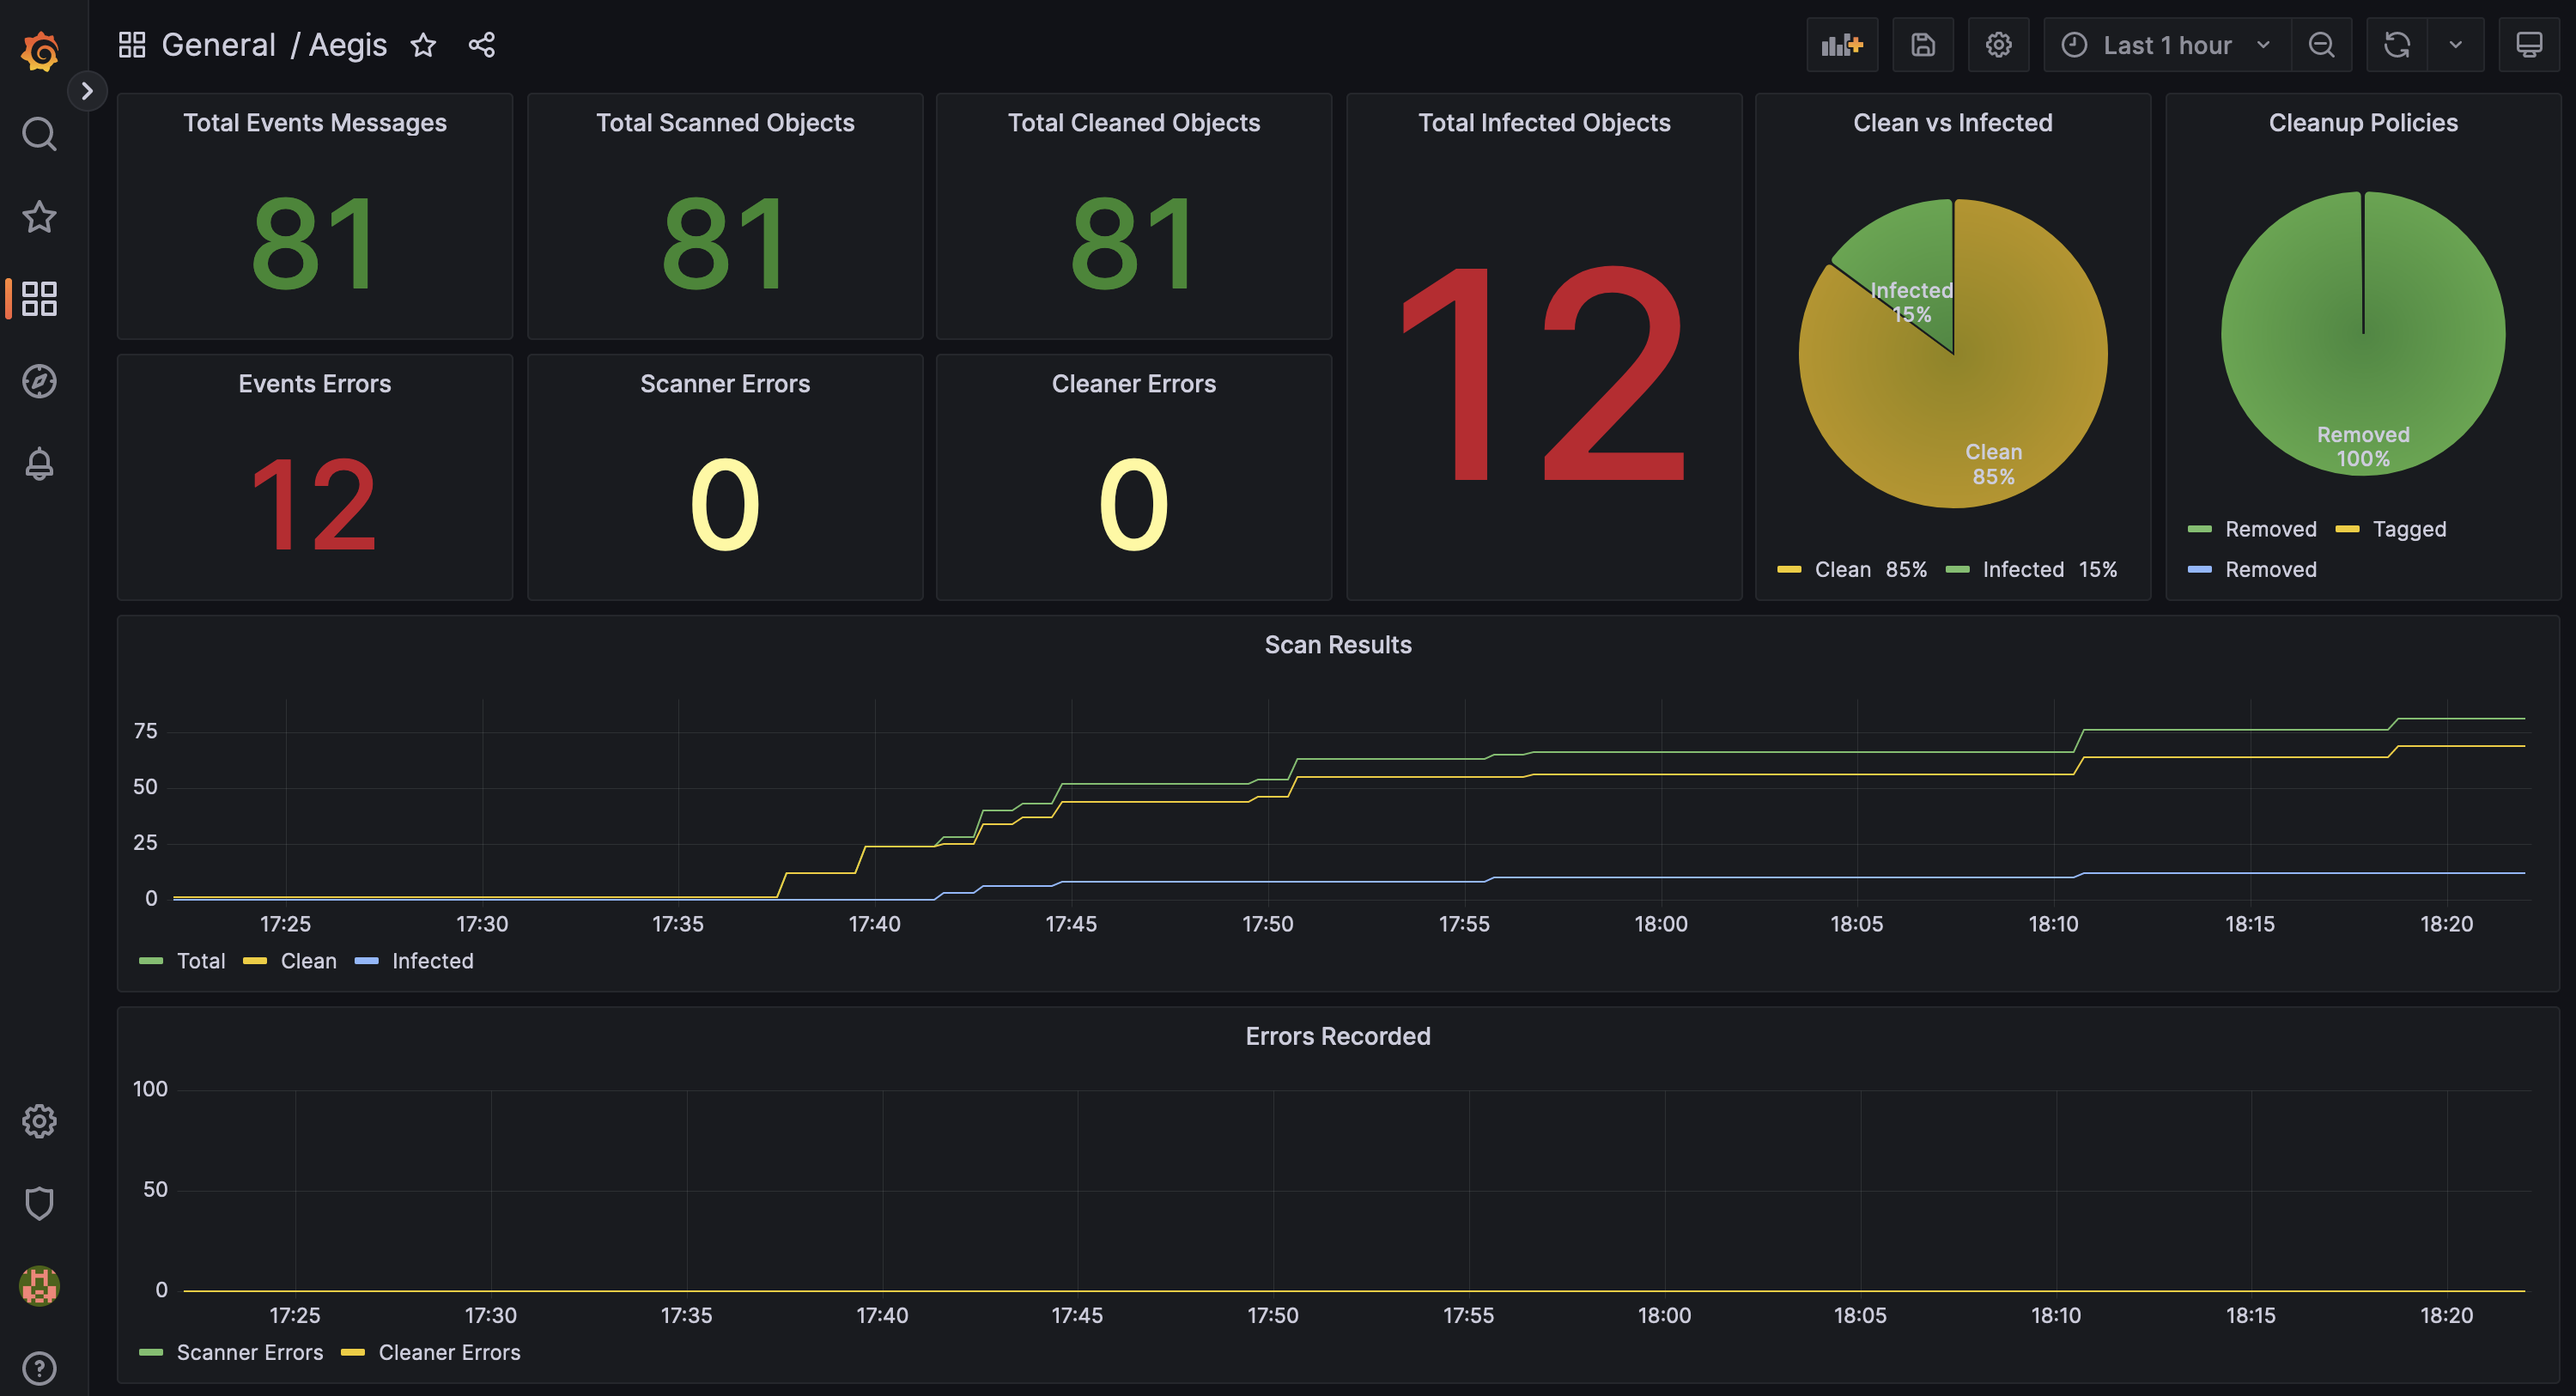
\includegraphics[scale=0.31]{images/grafana.png}
  \caption{An Example Grafana Dashboard}
  \label{fig:grafana}
\end{figure}

\subsection{Performance Evaluation}
\paragraph{}

% - [ ] Evaluate performance of the service
%   - [ ] Setup time
%   - [ ] Scan time
%   - [ ] Memory usage
%   - [ ] CPU usage
%   - [ ] Object size limits
% Eval
% Shutdown no loss
% No errors
% 100% detection
% Large file sizes
% Number of files

To access the performance of the solution, various metrics can be used. Many of
these are already available using Prometheus and Grafana. However, extra metrics
will be collected to aid the evaluation process. All of the metrics collected
were gathered from consumer grade hardware that is not fit for a production
environment. This will negatively impact the performance of the solution and
should be taken into account when evaluating the results. For this evaluation,
the cluster is deployed on an Apple M1 Macbook Pro with 16GB of RAM and a 10
core CPU giving 10GB and 8 cores to Docker.

\subsubsection*{Setup Time}
\paragraph{}

This metric is less important as it is only performed once. However, it is still
valuable for our analysis as it represents the time taken to deploy the a single
node in a cluster. This is measured from the time the \texttt{make create-node}
to first being able to perform a scan in Table \ref{tab:setup_timings}. This
includes the time taken to download the virus signature database.

\begin{table}[H] \centering
  \begin{tabular}{|l|l|}
    \hline
    \textbf{Setup Task}             & \textbf{Time mm:ss} \\ \hline
    Cluster started                 & 00:00         \\ \hline
    Cluster building complete       & 00:20         \\ \hline
    Docker Image pulled             & 00:27         \\ \hline
    Dependency repositories checked & 01:39         \\ \hline
    Dependencies downloaded         & 02:40         \\ \hline
    Pods starting                   & 04:41         \\ \hline
    Aegis first online              & 06:42         \\ \hline
    MinIO online                    & 11:13         \\ \hline
    Kafka online                    & 14:31         \\ \hline
    Virus database downloaded       & 16:38         \\ \hline
    First scan performed            & 16:45         \\ \hline
  \end{tabular}
  \caption{Cluster Setup Times}
  \label{tab:setup_timings}
\end{table}

The majority of the working time is waiting for the dependencies to come online,
namely ClamAV to download its virus signature database. Aegis is the first pod
to come online but enters into CrashLoopBackOff until all other pods are online.

\subsubsection*{Scan Throughput}
\paragraph{}
Over a longer period of time, the scan throughput can be measured. This could be
interpreted as two separate metrics, the total number of files scanned and the
total size of files scanned. Both are valuable metrics to measure to access the
sustained performance of the solution. Calculating throughput in Equation
\ref{eq:throughput} can be done by uploading a known number of files with a
known size and measuring the time taken to complete the scan. The results from
scanning a two folders, containing various media types, will be added in the Table
\ref{tab:scan_throughput} with average throughput calculated.

\begin{equation}
  \label{eq:throughput}
  Throughput = \frac{Total\ Scanned\ Size}{Time\ Taken}
\end{equation}

\begin{table}[H] \centering
  \begin{tabular}{|l|l|l|l|}
    \hline
    \textbf{Metric}       & \textbf{Folder 1} & \textbf{Folder 2} & \textbf{Average Throughput}\\ \hline
    Files Scanned         & 280          &   1218         & 1.48 Files/s        \\\hline
    Size of Files Scanned & 7370MB       &   7200MB       & 14.37 MB/s \\
    \hline
  \end{tabular}
  \caption{Scan Throughput}
  \label{tab:scan_throughput}
\end{table}

Folder one took 8.5 minutes and folder two took 8.4 minutes to complete.
Overall, the system is able to scan at the rate of 14.37MB/s or 50.5GB/h. For a
single node setup this is a good result as this covers the average network speed
of most home users. However, scaling up of the hardware is need for it to
achieve evaluate the full performance capabilities of the solution. The number of
files per second is less informative as the folder used contained a multitude of
different file sizes and types therefore is not a good representation of the
performance.

\subsubsection*{Scan Speed}
\paragraph{}
Unfortunately the intended inclusion of a scan time metric through Prometheus
became out of scope. However, calculating the scan speed can still be done using
the output logs from Aegis. This can be done as scan time is logged for each
file scanned, it is just not collected. Using a grep and awk in Figure \ref{fig:scan-time-commands}, all scan times
can be extracted and averaged to give the average scan time.

\begin{figure}[H]
  \begin{lstlisting}
    kubectl logs aegis-d564b7ddb-fvvmj | \
    grep -o 'Time: [0-9]*.[0-9]* sec' | \
    awk '{ for (i=1; i<=NF; i++) { sum+=$i; count++ } } END { print sum/count }'
    79.4085
  \end{lstlisting}
    \caption{Calculate Scan Time Commands}
    \label{fig:scan-time-commands}
\end{figure}

The result of 79.4085 seconds is a very long amount of time. This result was
from a system under maximum load on restricted hardware. If the same commands
are run on a system not under constant load the results change dramatically. For
a single scan, time taken is at 0.39 seconds. This shows that very quickly the
antivirus engine gets overwelmed by a queue of files to scan.

\subsubsection*{Scan Lag}
\paragraph{}
Scan lag is the time taken between uploading file and its scan completing. This can
be visualised by measuring the time taken between receiving a put event and
the scan completing. Grafana can be used to generate this graph as shown in the
Figure \ref{fig:scan-lag}. Note the folder used is different to the one used in the
previous example.

\begin{figure}[H]
  \centering 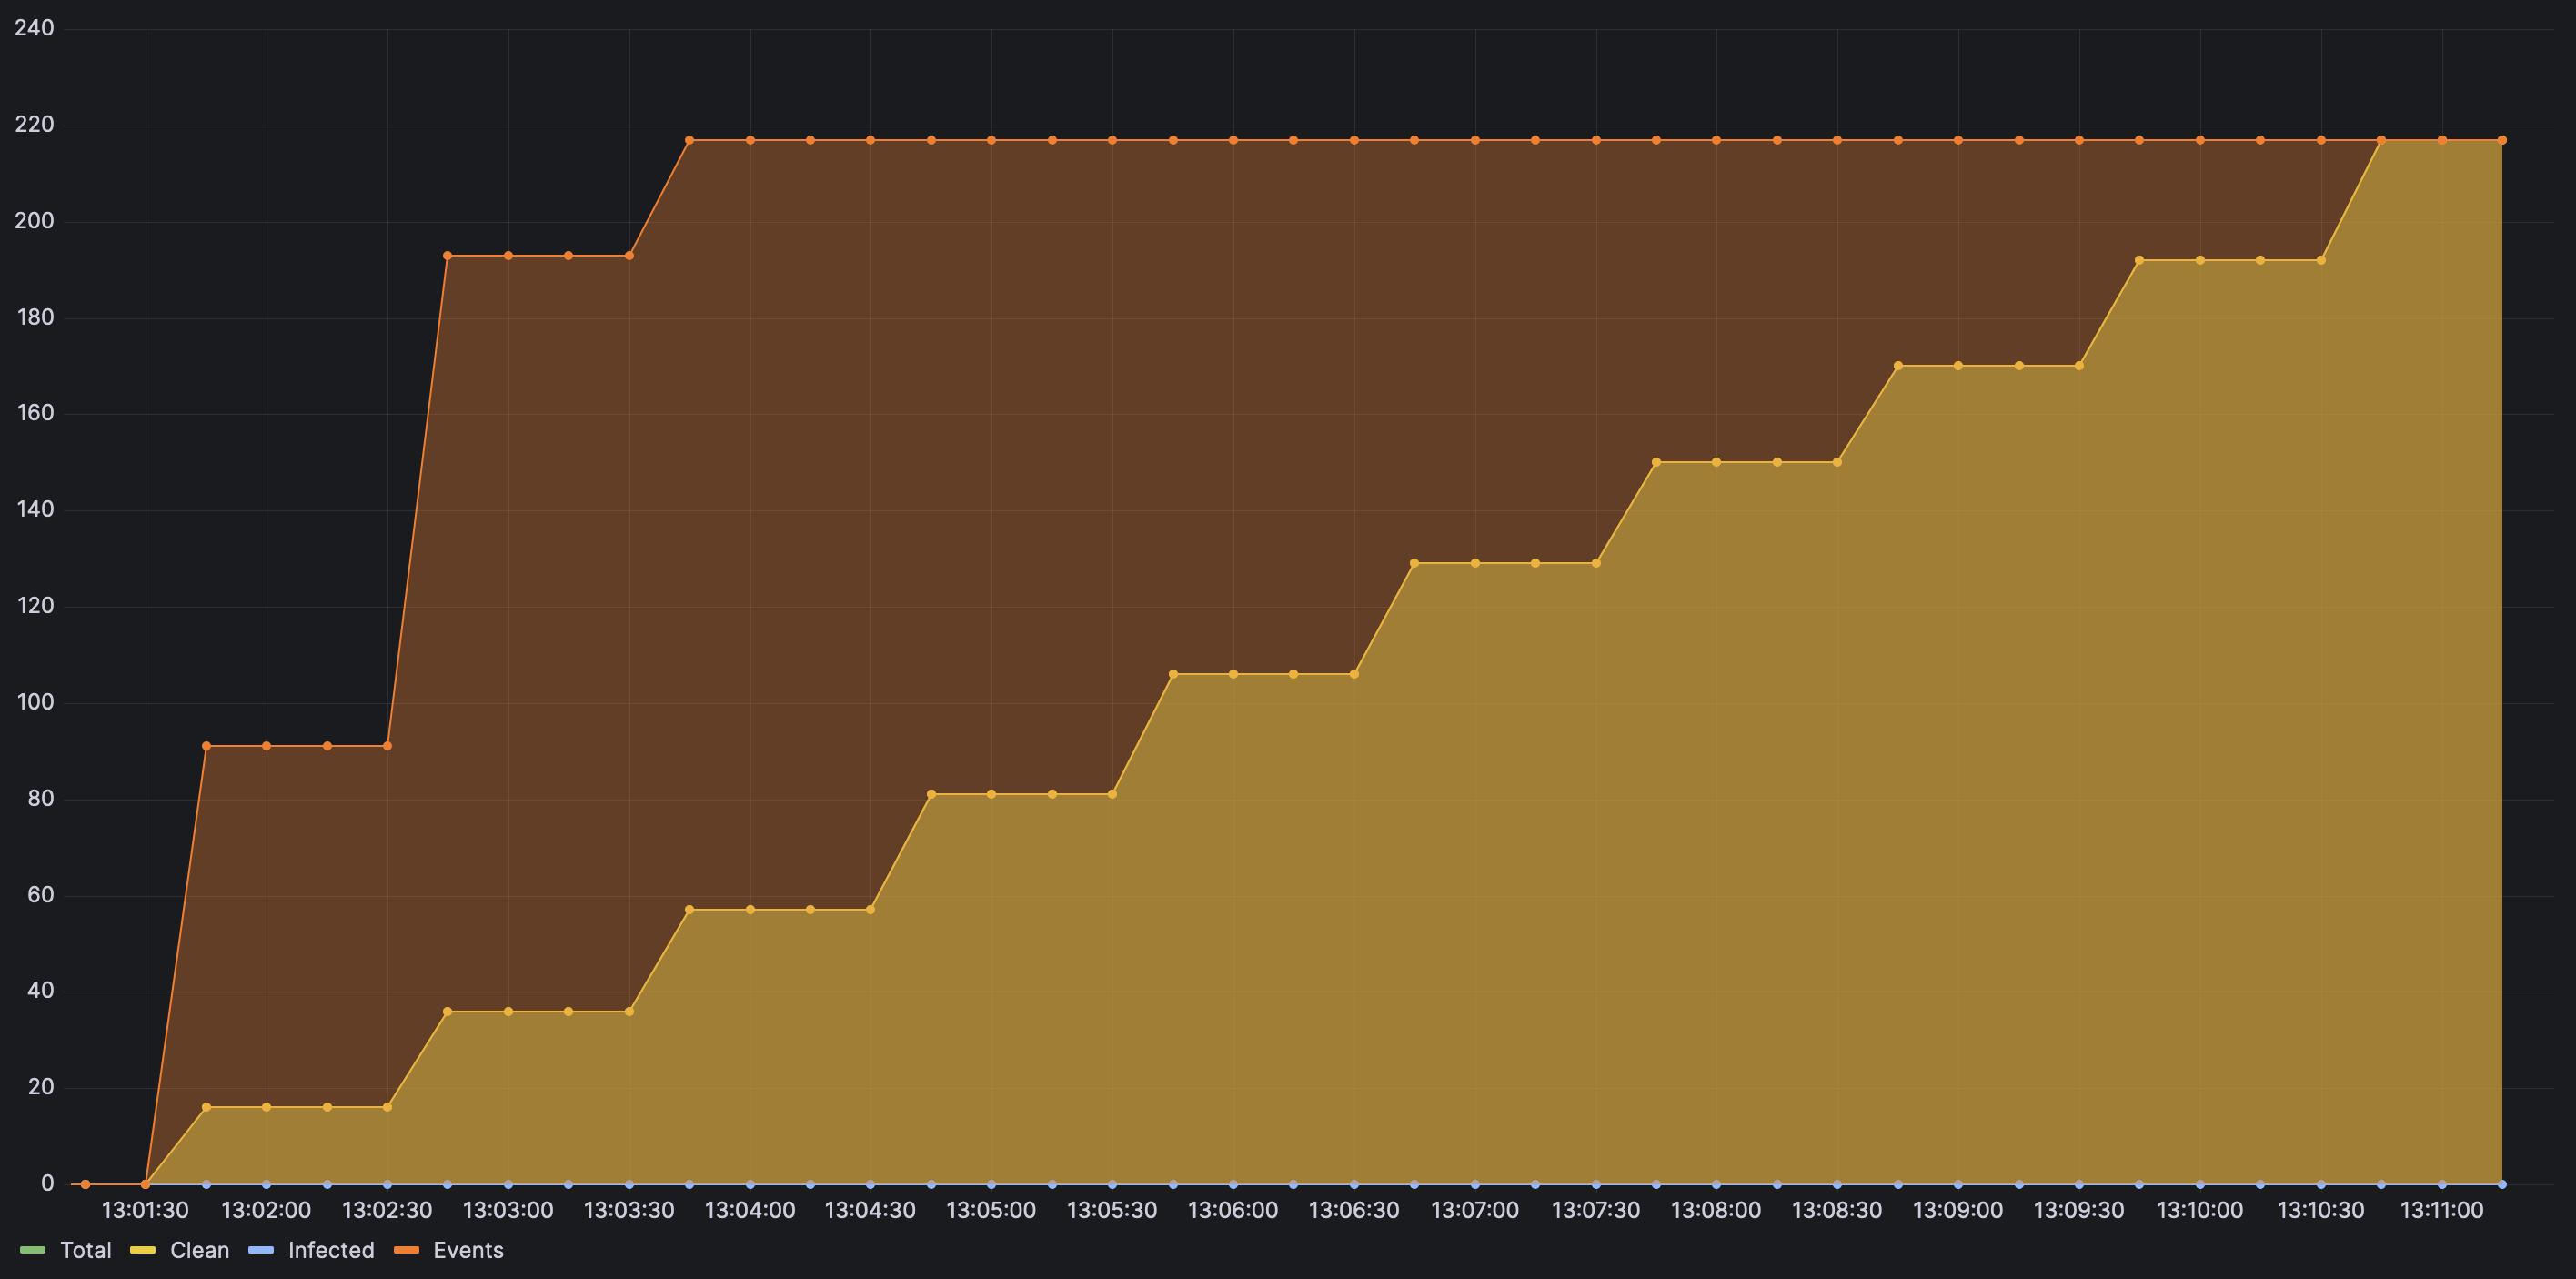
\includegraphics[scale=0.31]{images/scan-lag.png}
  \caption{Scan Lag Graph - Scans vs Time}
  \label{fig:scan-lag}
\end{figure}

This figure shows that there is a moderate amount of scan lag. This is due to
the high scan request load and the intensive nature of virus scanning against
large signature databases. In the graph the orange areas represents scan lag.
This is the time difference between Aegis receiving a put event and the scan
completing. The yellow area is the current scan progress. Overtime, the yellow
area matched the orange area as all the scan requests are processed. With the
process starting at 13:01:30, the peak of the orange area is at 13:03:45 which
is only 2m:15s after the first upload. The peak yellow area is at 13:10:45 showing
that it took a total of 9m:15s to complete the scan of the whole folder, a
difference of 7 minutes scan lag time. Its worth noting that the processing of
the scan requests is linear meaning that the process is never being bottlenecked
at any point. This backs up the previous assumption that the evaluation is
limited by hardware and not the capabilities of the solution.

If the users upload rate to MinIO stays below 14.37MB/s, the scan lag should be
minimal as the scan will be able to keep up with the upload rate. However, if
the upload rate exceeds this, the incoming scans will start to queue up and scan
lag will increase exponentially.

\subsubsection*{Scan Reliability}
\paragraph{}
Throughout the performance evaluation above, Grafana has displayed a running
total of all scan requests, scanned files and any error occurred in Figure
\ref{fig:scan-reliability}. This is a good indicator of the reliability of the
solution as no scans are being missed and no errors have been recorded.

\begin{figure}
  \centering 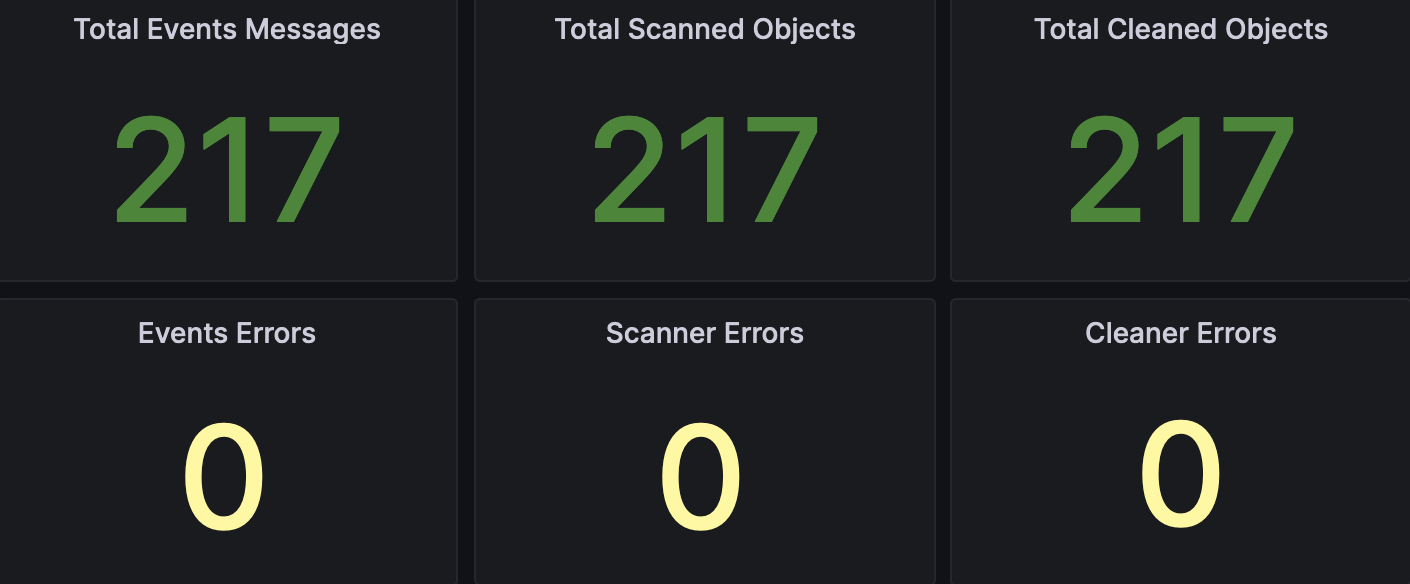
\includegraphics[scale=0.31]{images/scan-reliability.png}
  \caption{Scan Reliability}
  \label{fig:scan-reliability}
\end{figure}

\subsubsection*{Scan Accuracy}
\paragraph{}
Scan accuracy is redundant to measure as the solution only uses ClamAV to scan
files. If higher accuracy than what ClamAV provides is required, adding more
antivirus engines is possible with the aggregate scan results being determined
by the union of positive scan results \citep{av-comparison}. This is shown in Figure
\ref{scan-union}.

\begin{figure}[H]
  \centering 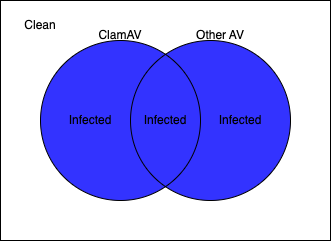
\includegraphics[scale=0.45]{diagrams/scan-union.png}
  \caption{Combined AV Effectiveness}
  \label{scan-union}
\end{figure}


\subsubsection*{Shutdown Reliability}
\paragraph{}
During an unexpected error or graceful shutdown process, reliably stopping the
scanning process is essential to ensure that no files are left unprocessed. To
evaluate this, a set of scans will be requested with known malicious files.
These files should be removed under the corresponding cleanup policy and
therefore no files should be left in the object store. Mid-scan, an interrupt
signal will be given to Aegis causing it to enter graceful shutdown. The results
of running the test are available in the appendix in Listing
\ref{appendix:shutdown-logs}.

As expected, zero files are left in the object store after Aegis had restarted
and continued processing the scan requests. This shows that there are no gaps in
the execution of the solution if any error conditions would occur.

\subsection{Comparing Functional Requirements}
\paragraph{}
By comparing the functional requirements defined at the beginning of the report,
a conclusion can be made on whether the solution has met the requirements. Each
requirement is evaluated in Table \ref{tab:functional-reqs-evaluation}.

\begin{table}[H]
  \centering
  \begin{tabular}{|p{0.3\textwidth}|p{0.7\textwidth}|}
    \hline
    \textbf{Requirement} & \textbf{Evaluation} \\ \hline
    Provide a way of detecting the latest uploads to the object store. & This
                                                                        requirement
    has been achieved. Kafka has been successfully connected to MinIO and can
                                                                        read all
    put events given by MinIO. It can also hold events if Aegis is not ready to
                                                                        receive
                                                                        scan
                                                                        requests
    in the event of an error or shutdown. \\ \hline
    Record the results of the malware detection within the object store. &
                                                                          Provided
                                                                          are
                                                                          three
                                                                          cleanup
    policies, remove, tag or quarantine. This requirement has been met and over
                                                                          achieved
    as there are multiple options for the user to choose from. \\ \hline
    Provide the ability to measure key performance and analytic metrics. & As shown by
                                                     \ref{fig:grafana}, various
                                                     metrics have been collected
    throughout the Aegis' lifetime. These have also been consumed and
                                                     analysis has been
                                                     performed. This requirement
    has been met. \\ \hline
    Scale alongside MinIO to ensure that it does not bottleneck the object store
    at high loads. & This requirement has been partially met. Aegis never
                    bottlenecks the object store during execution due to the use
    of an event queue. However, Aegis does not effectively scale with MinIO to
                    keep up with the incoming uploads. \\ \hline
    Provision for future expansion and ongoing maintenance. & The solution fully
                                                             meets this
                                                             requirement for
                                                             many reasons.
                                                             Firstly, structured
                                                             logging,
                                                             configuration files
                                                             metric collection
                                                             and audit logging
                                                             means that
                                                             active maintenance
                                                             of the solution
                                                             should be as easy
                                                             as possible. In
                                                             addition, Aegis has
                                                             been designed to be
                                                             as extensible as
                                                             possible with room
                                                             for multiple types
                                                             of scanning
                                                             workflows and
                                                             multiple antivirus engines.
    \\ \hline
    Must be cost effective and legally viable for commercial use. & This
                                                                    requirement
                                                                    has been met
                                                                    as all
                                                                    external
                                                                    software
                                                                    used is
                                                                    open-source
                                                                    and freely
                                                                    available.
                                                                    If in
                                                                    production
                                                                    use,
                                                                    additional
                                                                    antivirus
                                                                    engines are
                                                                    used then
                                                                    paid
                                                                    software can
                                                                    be included.
    \\ \hline

    \hline

    Have a high level of customisability to allow for different use cases. &
                                                                             This
                                                                             requirement
    has been met as a configuration file is available for Aegis that allows
                                                                             customisation
                                                                             of
                                                                             all
    endpoints, name of the topic, database details, the cleanup policy and make
                                                                             more.
                                                                             There
                                                                             is
                                                                             also
                                                                             room
                                                                             to
                                                                             add
                                                                             different
                                                                             types
                                                                             of
                                                                             scanning
                                                                             workflows
                                                                             and
                                                                             antivirus engines.
  \\ \hline
    Allow for efficient and transparent debugging in the event of failure. & Structured
    logging is included that provides insightful feedback at various levels. In
                                                                             addition,
    metric collection and audit logging make it easy to keep track of errors and
    scan history. Including a log aggregation tool, such as Splunk, could
                                                                             improve
                                                                             the
    satisfaction of this requirement. \\ \hline

    Add more complex metrics - Histogram, Gauges, etc. & Although many useful
                                                        metrics are collected,
                                                        no complex metrics have
                                                        been added. These have a
    minimal impact on the overall solution so have not been prioritised. \\ \hline \hline
    Provide the choice of multiple antivirus engines. & No other antivirus
                                                       engines have been added
                                                       to the solution. However,
    the structure is in place to allow for additions in the future.\\ \hline
    Provide a warning when under ``delete'' cleanup policy. & This requirement
                                                              was partially met
                                                              as selecting the
                                                              delete policy is
                                                              done within the
                                                              \texttt{config.env}
    file. In the file a commented warning is provided. In the future, if the
                                                              configuration is
                                                              available via GUI
                                                              this requirement
                                                              would move up in
                                                              priority from
                                                              could to should. \\ \hline
    Automatically setup bucket notifications to be sent to the event queue. & In
    practice, manually setting up the solution must only be done once. This lead
    the decision that thorough documentation was a better use of the limited
                                                                              time
                                                                              available.
    \\ \hline
    Supply the MinIO policies the solution will use e.g. ``put'' and ``get''. &
   This requirement is relatively simple but has remained out of scope. This
                                                                                will
                                                                                need
    to be completed to be fully production-ready to provide information to
                                                                                inform
                                                                                any
                                                                                future
                                                                                users
                                                                                of
                                                                                the
                                                                                access
                                                                                it requires
                                                                              \\ \hline \hline

    Prevent the downloading of files if flagged as infected. & This requirement
                                                              was not met as it
                                                              involved making
                                                              changes to the
                                                              MinIO web console.
    This was determined to be out of scope due to the additional time required
                                                              to research the
                                                              implementation for
    a insignificant change to the solution. \\ \hline
    Protection from ``inside man'' attacks. & No protection from ``inside man''
                                              attacks has been added. This is
                                              still not a priority for systems
                                              where users will have a wide range
    of abilities already, such as deleting or reading files. \\ \hline
    Provide multiple types of scanners e.g. hash or server based AV scanner. &
                                                                               Only
                                                                               a
    single workflow for scanning files has been provided. However, provisions
                                                                               for
                                                                               implementing
    this in the future has been put into place, if required.  \\ \hline
  \end{tabular}
  \caption{Functional Requirements with Evaluation}
  \label{tab:functional-reqs-evaluation}
\end{table}

\subsection{Comparing Non-Functional Requirements}
\paragraph{}
Additionally, the non-functional requirements have been evaluated in the table
\ref{tab:non-functional-reqs-evaluation}.

\begin{table}[H]
  \centering
  \begin{tabular}{|p{0.1\textwidth}|p{0.9\textwidth}|}
    \hline
    \textbf{Requirement} & \textbf{Evaluation} \\ \hline
    Speed & As seen in the scan throughput section, if the incoming scan
            requests stays at or below 14.37MB/s, then the solution will keep up
    with MinIO. However, it suffers dramatically under high load with average
            scan times rising to 79. This is does not satisfy this requirement
            under maximum throughput conditions. In a less intensive
            scenario, scans are performed within 0.39 which is a very good
            result. More focus in the future should be placed on quickly scaling
    out the antivirus engines to meet high demand.\\ \hline
    Scalability & The solution lacks to achieve this requirement. Provisions for
          scaling out have been added but the scope constraints prevented them
                  from being fully implemented. This negatively affects the
                  project as this requirement was a priority. \\ \hline
    Availability & Scan reliability has shown that throughout benchmarking the
                   cluster has not become unavailable. While object store
                   availability is the responsibility of MinIO, the stability of
    the cluster is apart of the solution. As there were no unexpected downtime,
                   this requirement has been met. \\ \hline
    Reliability & The reliability of the solution has proven to be good. No
                  unexpected errors happened during the evaluation process. When
    performing a test of Aegis' graceful shutdown procedure, zero files were
                  left unprocessed.\\ \hline
    Capacity & As Aegis only uses one temporary cache file, the maximum capacity
               needed can be calculated by multiplying the average throughput by
               the average scan time. This results in an average capacity
               required as $14.37$MB/s x $79.4$s$ = 1.14$GB. This is
               highly achievable for the majority of production environments. \\ \hline
    Security & The security of the system is largely reliant on MinIO's built-in
    authentication. This stops unwanted puts / gets from the system without
               Aegis getting involved. All files scanned do not leave the
               cluster and therefore are sheltered from external access. \\ \hline
    Privacy & As the scanned files remain inside of the cluster, privacy is
    preserved. In addition, the only metrics collected are counting occurrences
              and never interpret the contents of any file. ClamAV does look at
              internal contents but apart from virus signature database
              downloads, does not have any outside access. \\ \hline
  \end{tabular}
  \caption{Non-Functional Requirements with Evaluation}
  \label{tab:non-functional-reqs-evaluation}
\end{table}

\subsection{Project Aims Evaluation}
\paragraph{}

Upon reviewing the functional and non-functional requirements, it can be said
that the project aim of "implementing malware detection into MinIO without
compromising the platform's scalability or performance" has been achieved to
some extent. While a malware detection component has been successfully
integrated, certain compromises were required to remain within the project
scope. The current solution does not dynamically scale the antivirus engines in
response to increased demand on the object store, resulting in substantial scan
latency that could potentially affect user experience.

Despite this, the developed solution serves as a solid foundation for a
production-grade malware detection system for MinIO, boasting high availability,
reliability, and security. With further time and resource investment, it has the
potential to scale efficiently alongside MinIO without compromising performance.

Through the course of this project, I have made significant strides towards
achieving my personal aims. Specifically, I have successfully deepened my
understanding of the Go programming language and the MinIO platform. Creating a
complete and high quality Go application has taught me the value of effective
design architecture to maximise cohesion and minimise coupling. At a few points
in the project, refactoring was required which could have been avoided with
a more informed planning phase.

Furthermore, I have increased my experience in designing and implementing
production-ready solutions within a microservice environment. Through the
practical application of microservice design principles and deployment
strategies, I have gained insights into the complexities and rewards of this
architectural style.

Yet, perfecting the management of time, scope, and resources in large-scale
projects remains a field needing more development. The wide scope of this
project introduced considerable challenges, such as juggling competing
priorities and resolving unforeseen issues. Even with these challenges, it
illuminated the vital importance of effective project management skills and has
motivated me to target continued growth in this area.

\subsection{Testing Evaluation}
\paragraph{}
In Aegis, every internal package is accompanied by a set of unit tests. These
tests can be executed using the Go CLI, and their coverage varies across
different packages. The overall test coverage for Aegis is a good indicator of
the effectiveness of the tests in place. This also supports the reliability of
the solution as errors should be caught before deployment.

The average test coverage for Aegis is 64\%. Supplied in the appendix in the
output from performing the tests in Listing \ref{appendix:go-tests}.

For future development, achieving 100\% coverage over all packages is a worth
while goal, especially to claim production-ready status. This will ensure that
every piece of code is thoroughly tested, improving the overall robustness and
reliability of the system. One way to achieve this is through test-driven
development (TDD), a software development methodology that involves writing
tests before implementing the actual code. By adopting TDD, testing becomes the
priority, and each package's level of quality and encapsulation will be
constantly assessed, therefore catching more errors before deployment.


\section{Product Issues / Future work} % What you would do next time
\paragraph{}

Although the solution is working, it is not without its limitations. From the
evaluation, two categories of issues have been identified. Firstly, the hard
constraint of the project deadline has meant that some features have not been
implemented or compromises have had to be made. This will have negatively
affected the quality of the solution These issues are listed below.

\begin{itemize}
  \item Lack of scalability from load balancing antivirus engines. This impacts
        the scalability of the solution as no scanning can happen in parallel
        when the system is under load. This could be solved by implementing a
        horizontal pod auto-scaler to adaptively scale number of concurrent pods
        available based on the demand of compute resources \citep{scale-pods}.
  \item Diversify metric collection so that a larger range of metrics are
        collected. For example, the average scan time of a file and the average
        time a file is in the cache. This could provide more insights into the
        performance of the solution.
  \item The testing code coverage could be improved to achieve 100\% coverage
        for both internal and external pkg packages. This would ensure that all
        code going into production has had some level of testing. Using table
        driven tests could help improve the coverage of edge cases and error
        conditions \citep{table-driven-tests}.
  \item While the scanned files are removed (if AEGIS\_REMOVE\_AFTER\_SCAN is
        true), the sub-folders under the buckets are not. This is a hard issue
        to solve as it is possible to delete a folder while another file is
        being downloaded to it. The impact of retaining all folders is small as
        an empty folder uses minimal storage space but over time writing to the
        store could slow down. One possible solution is to store all files in a
        single folder. This could lead to naming conflicts which a UUID could
        solve \citep{UUID}. Another solution could be having a retention policy
        on each folder which would delete the folder after a given time or under
        a given condition.
  \item
\end{itemize}

Secondly, new opportunities have identified themselves during the development of
the solution. These could be implemented in future projects related to this
area. Below is a list of the issues identified.

\begin{itemize}
  \item MinIO has the ability to integrate Audit logging and Prometheus metrics
        into its existing metric collection service. Combining the two could
        provide a more complete picture of the system to draw conclusions from.
  \item No feature tests have been written for this solution. Feature tests
        would test multiple packages together to ensure that the overall
        workflow of the system is correct. This testing would be valuable for
        ongoing production use.
  \item The solution only deploys to a single node cluster running on a single
        machine. In a production environment, this would not be the case and
        therefore more work is needed to ensure that the solution can be
        deployed to a multi node cluster.
  \item Using the MinIO web console, the results of the scan could be viewed. In
        addition, warning messages could be added to inform the user of infect
        files. Depending on the production use, this feature could be valuable.
  \item Store the scan result in metadata rather than tagging to improve
        immutability of tags. This might also raise the ability for bad actors
        to edit object metadata outside of MinIO.
  \item Unscanned files are currently not tagged with anything to indicate that
        they have not been scanned. This could be useful for auditing or user
        feedback purposes.
  \item Calculate the hash of a object, upon performing put, inside of MinIO
        using lambda functions \citep{minio-lambda}. This reduces the size of
        the download required to scan a file. However, removes the ability for any
        antivirus engine to use any fuzzy matching.
  \item Have a selection of ready-to-go antivirus engines that the user can
        choose from to improve overall scanning accuracy \citep{av-comparison}.
  \item Put tagging messages are ignored by the event queue. This could
        potentially cause a security issue where a change in tags are not
        scanned. The risk of this is minor as only a user with access to the
        system can modify the tag which could be classed as an inside man attack
        which was not in the scope of the project.
  \item Queue deduplication could be used to ensure that the same file is not
        scanned multiple times while in the event queue. This would improve the
        performance of deployments that are receiving a large number of puts
        involving the same file.
\end{itemize}

\section{Conclusions}
\subsection{}

As this project concludes, further work remains to ensure the solution aligns
with the standards delineated in the project specification. Despite making
considerable progress, the current solution does impact the scalability and
performance of the MinIO object store. However, it's important to recognize the
significant accomplishments of the project; the successfully development of a
microservice capable of scanning uploaded files for malware. The Aegis service
operates efficiently, requiring minimal cache for object scans and never acting
as a bottleneck in the workflow.

Moreover, the solution integrates numerous production-level features necessary
for enterprise deployment. It also maintains compatibility with existing MinIO
features, including erasure coding and object encryption. These successes affirm
the potential of the solution, even as we acknowledge areas that need further
development.

Additionally, throughout the development process, numerous potential research avenues have
been identified. Given more time, these could be thoroughly explored and
capitalised upon.

\section{Reflection on Learning}
\subsection{}

Throughout the course of this project, I have dramatically improved on my
knowledge and experience. The project provided a valuable opportunity for me to
further my understanding of the Go programming language and the MinIO platform.
The endeavor of creating a microservice application using Go was challenging at
points, but it served as an enriching exercise that will improve my grasp of
effective system design and software engineering principles.

Furthermore, the project has shown me the importance of various non-technical
skills when working on large-scale developments. Particularly, project
management skills were brought to the forefront given the broad requirements and
restrictive scope of the project. I have recognized the crucial role of
effective time management, clear goal-setting, and efficient resource allocation
in ensuring the project's success. While I did encounter a few setbacks, I
managed to adapt my approach and implement necessary changes to facilitate the
project's progression.

Despite the overall success of the project, I recognize that certain areas
require further refinement. Notably, maintaining the scalability and performance
of the MinIO object store while staying within scope present many issues.
Nevertheless, these hurdles have served as invaluable learning experiences,
offering insight into areas of potential future focus. Moving forward, I am
eager for another opportunity to apply the skills and knowledge I've gained from
this project to new challenges and projects.
\section{Appendix}

\begin{figure}[H]
  \centering 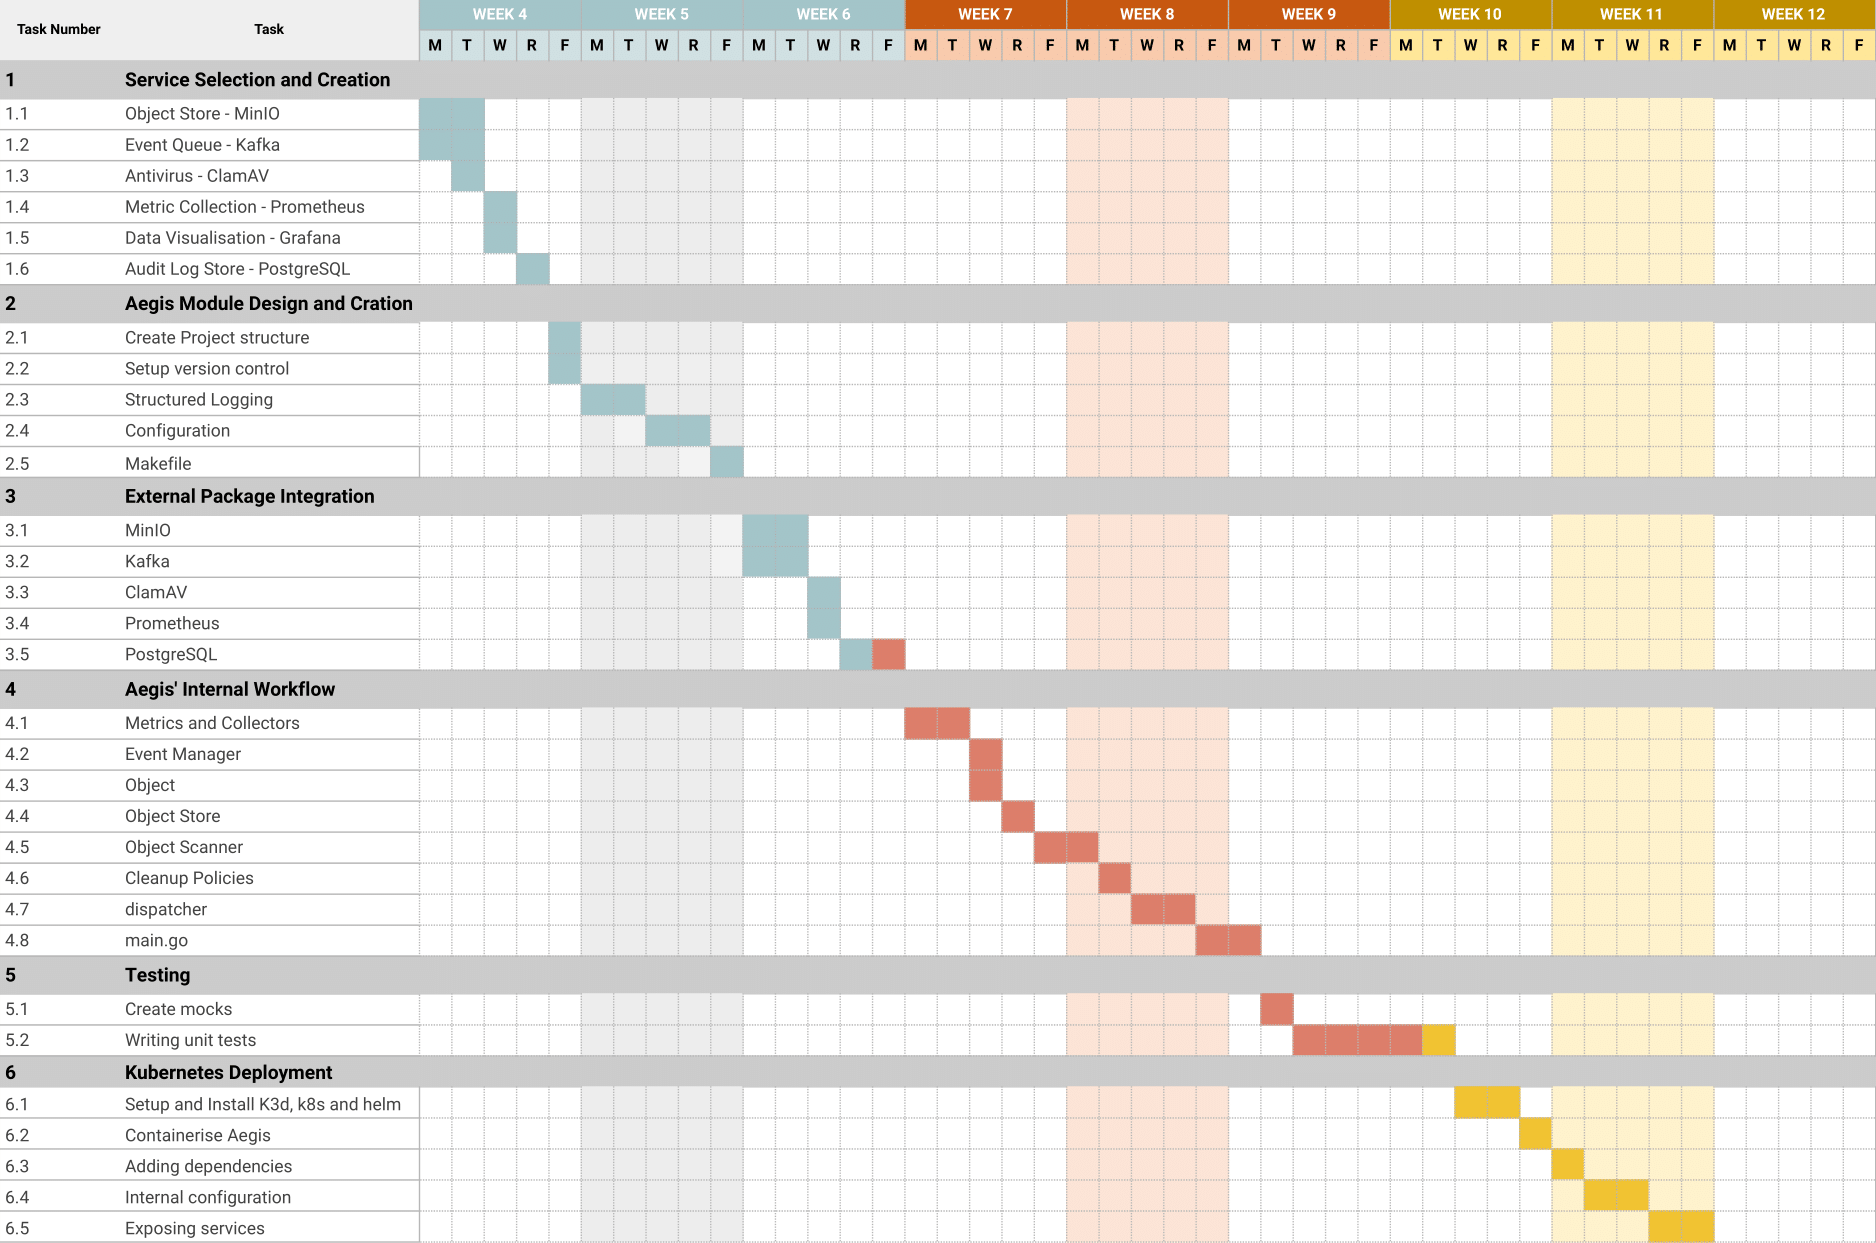
\includegraphics[scale=.67]{diagrams/gantt-chart.png}
  \caption{Timeline of Aegis' Development}
  \label{appendix:gantt}
\end{figure}

\begin{figure}[H]
  \centering 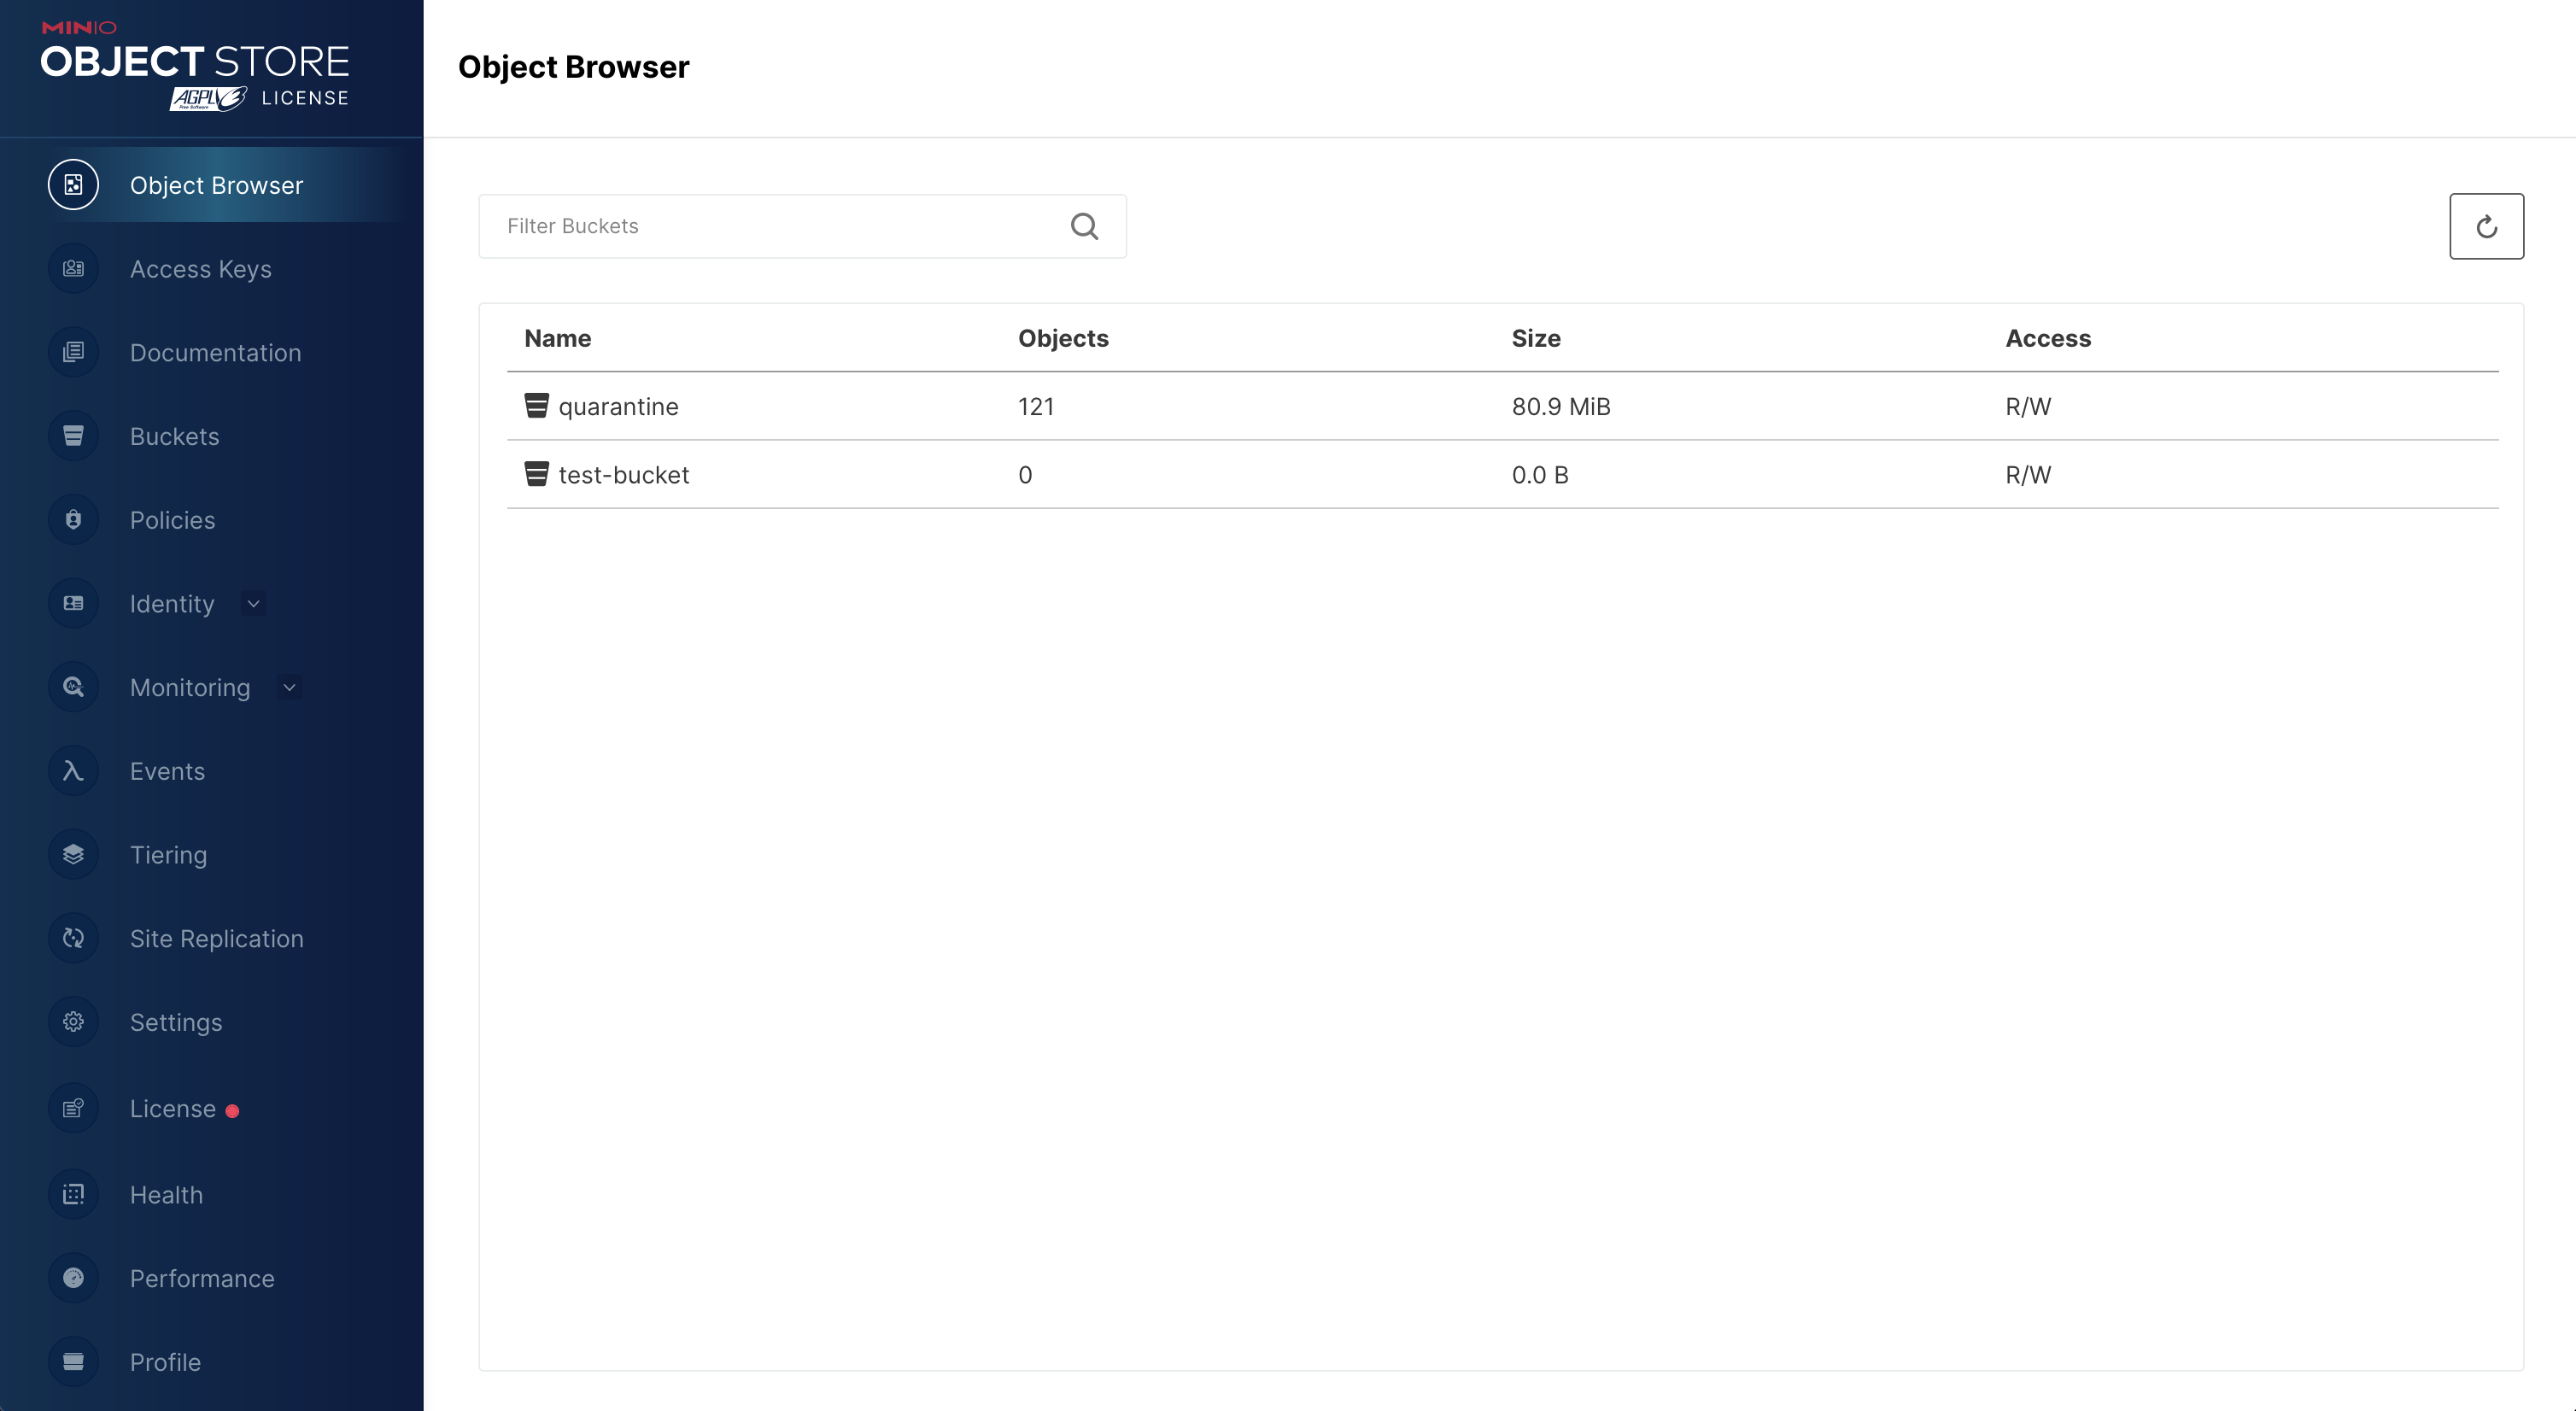
\includegraphics[scale=.3]{images/minio-console.png}
  \caption{Image of MinIO's Web Console}
  \label{appendix:minio-console}
\end{figure}

\begin{figure}[H]
  \centering 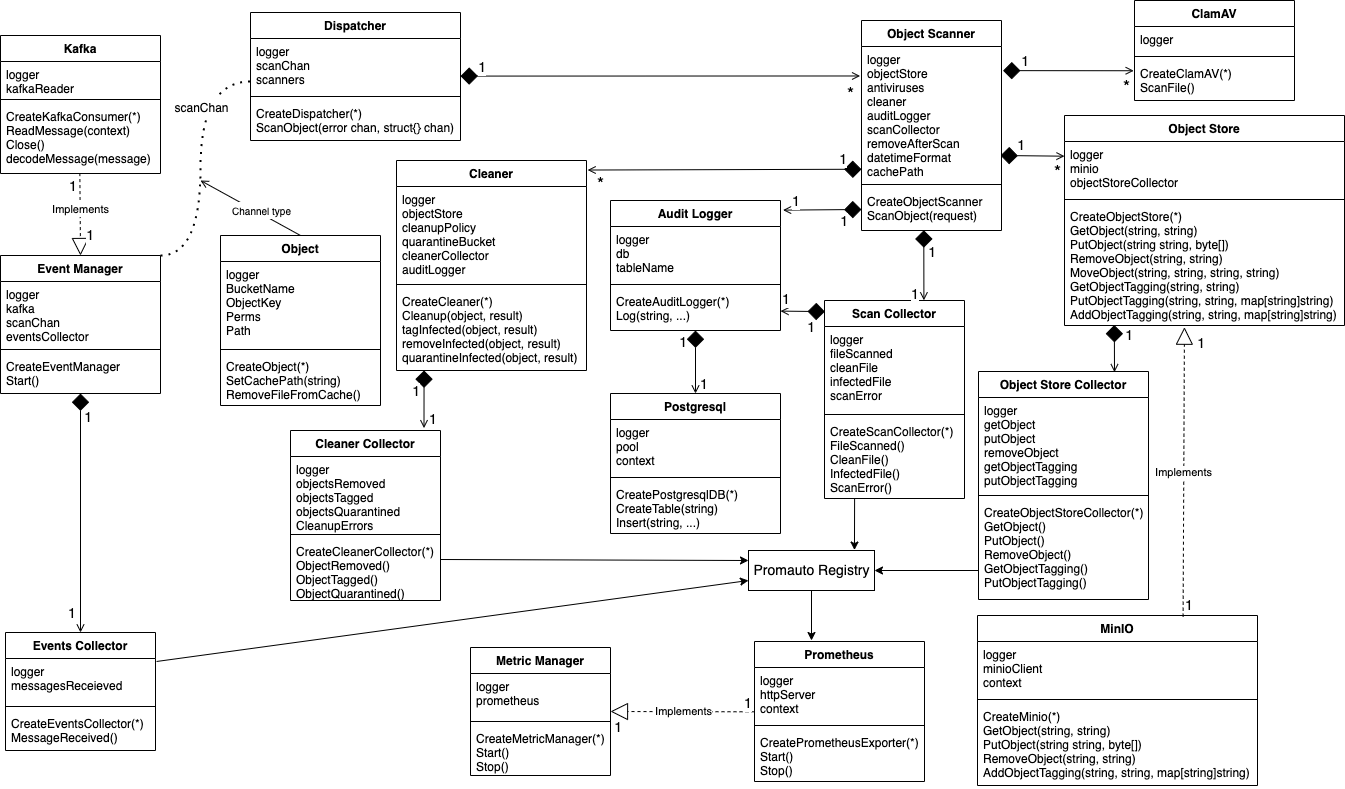
\includegraphics[scale=.38]{diagrams/class-diagram.png}
  \caption{Plan of Aegis' Internal Packages}
  \label{appendix:class-diagram}
\end{figure}

\begin{figure}[H]
  \centering 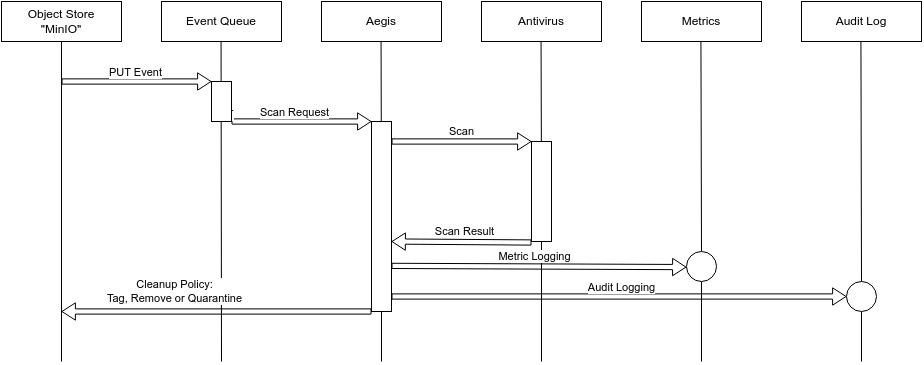
\includegraphics[scale=0.53]{diagrams/general-sequence.png}
  \caption{Aegis General Sequence Diagram}
  \label{appendix:general-sequence}
\end{figure}

\begin{figure}[H]
  \centering 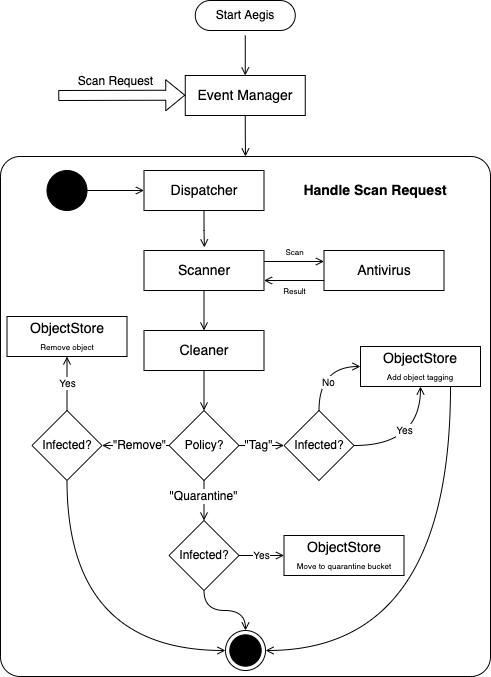
\includegraphics[scale=0.5]{diagrams/flow-diagram.png}
  \caption{Aegis Scan Request Flow Diagram}
  \label{appendix:flow-diagram}
\end{figure}

\begin{figure}[H]
  \centering 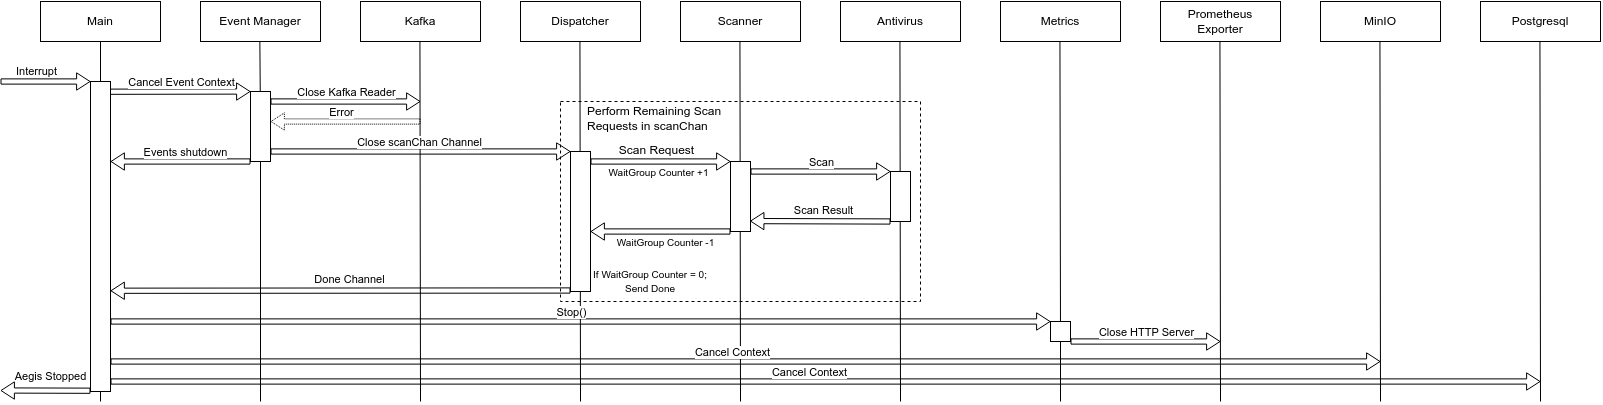
\includegraphics[scale=0.31]{diagrams/shutdown-sequence.png}
  \caption{Aegis Shutdown Sequence Diagram}
  \label{appendix:shutdown-sequence}
\end{figure}

\lstinputlisting[caption={Example Kafka Notification},
label=appendix:kafka-notif, numbers=left]{assets/example-notif.json}

\lstinputlisting[caption={Example Kafka Notification},
label=appendix:clamd-scan]{assets/example-clamd-scan.txt}

\lstinputlisting[basicstyle=\small,caption={Example Exposed Metrics},
label=appendix:example-exposed-metrics]{assets/example-exposed-metrics.txt}

\lstinputlisting[language=SQL, caption={Create Table SQL Query},
label=appendix:create-table-query]{assets/create-table-query.txt}

\lstinputlisting[language=SQL, caption={Insert into Table SQL Query},
label=appendix:insert-query]{assets/insert-query.txt}

\begin{figure}[H]
  \centering 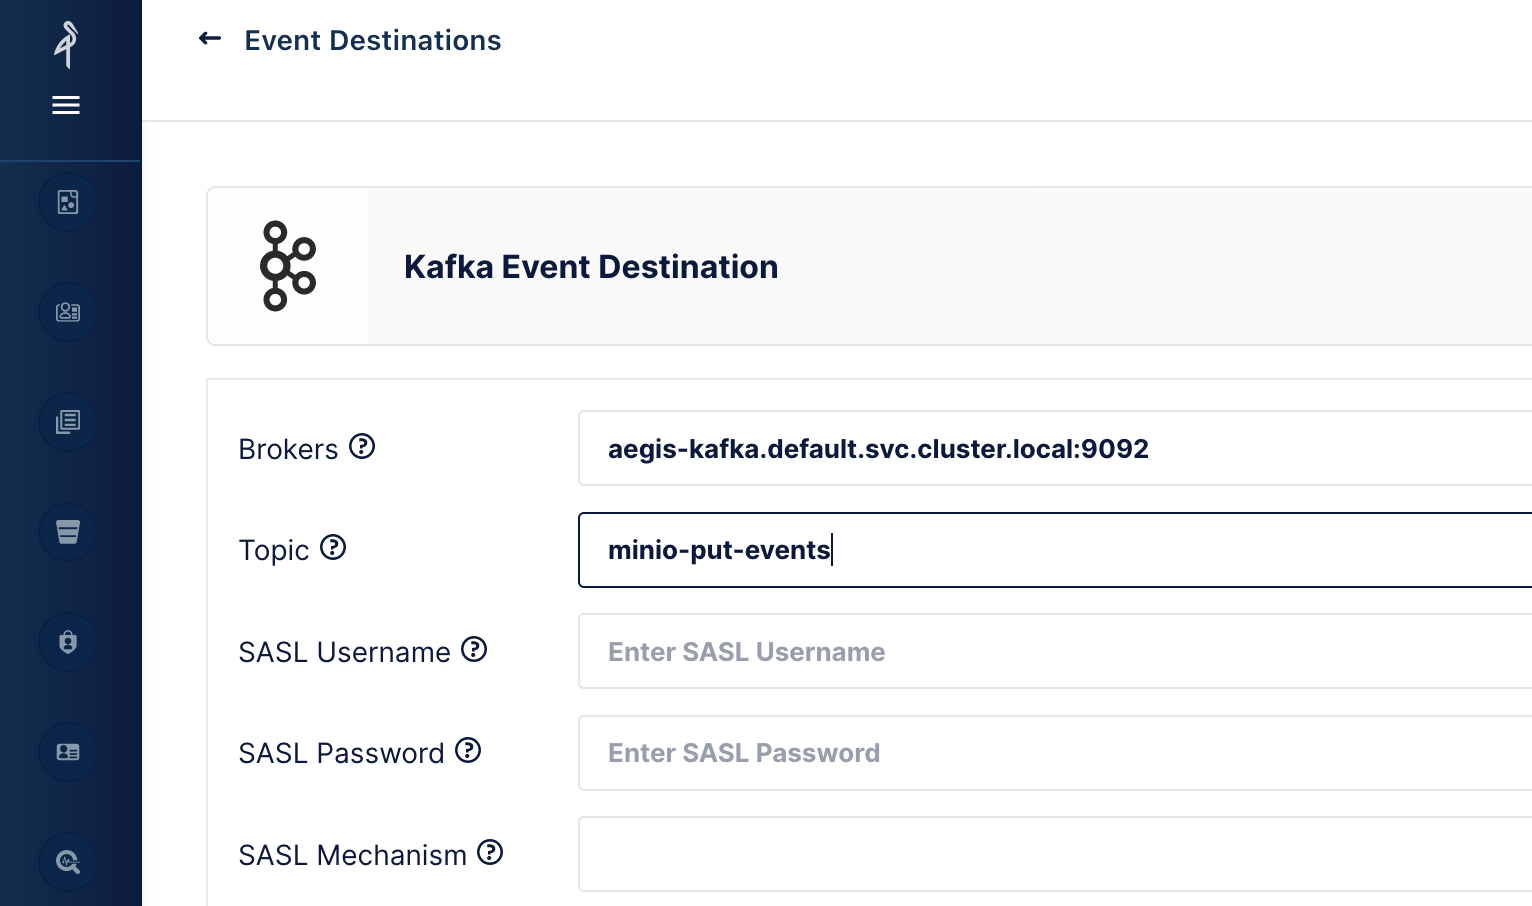
\includegraphics[scale=0.45]{images/minio-event-queue.png}
  \caption{Configuring MinIO to Send Events to Kafka}
  \label{appendix:minio-event-queue}
\end{figure}

\begin{figure}[H]
  \centering 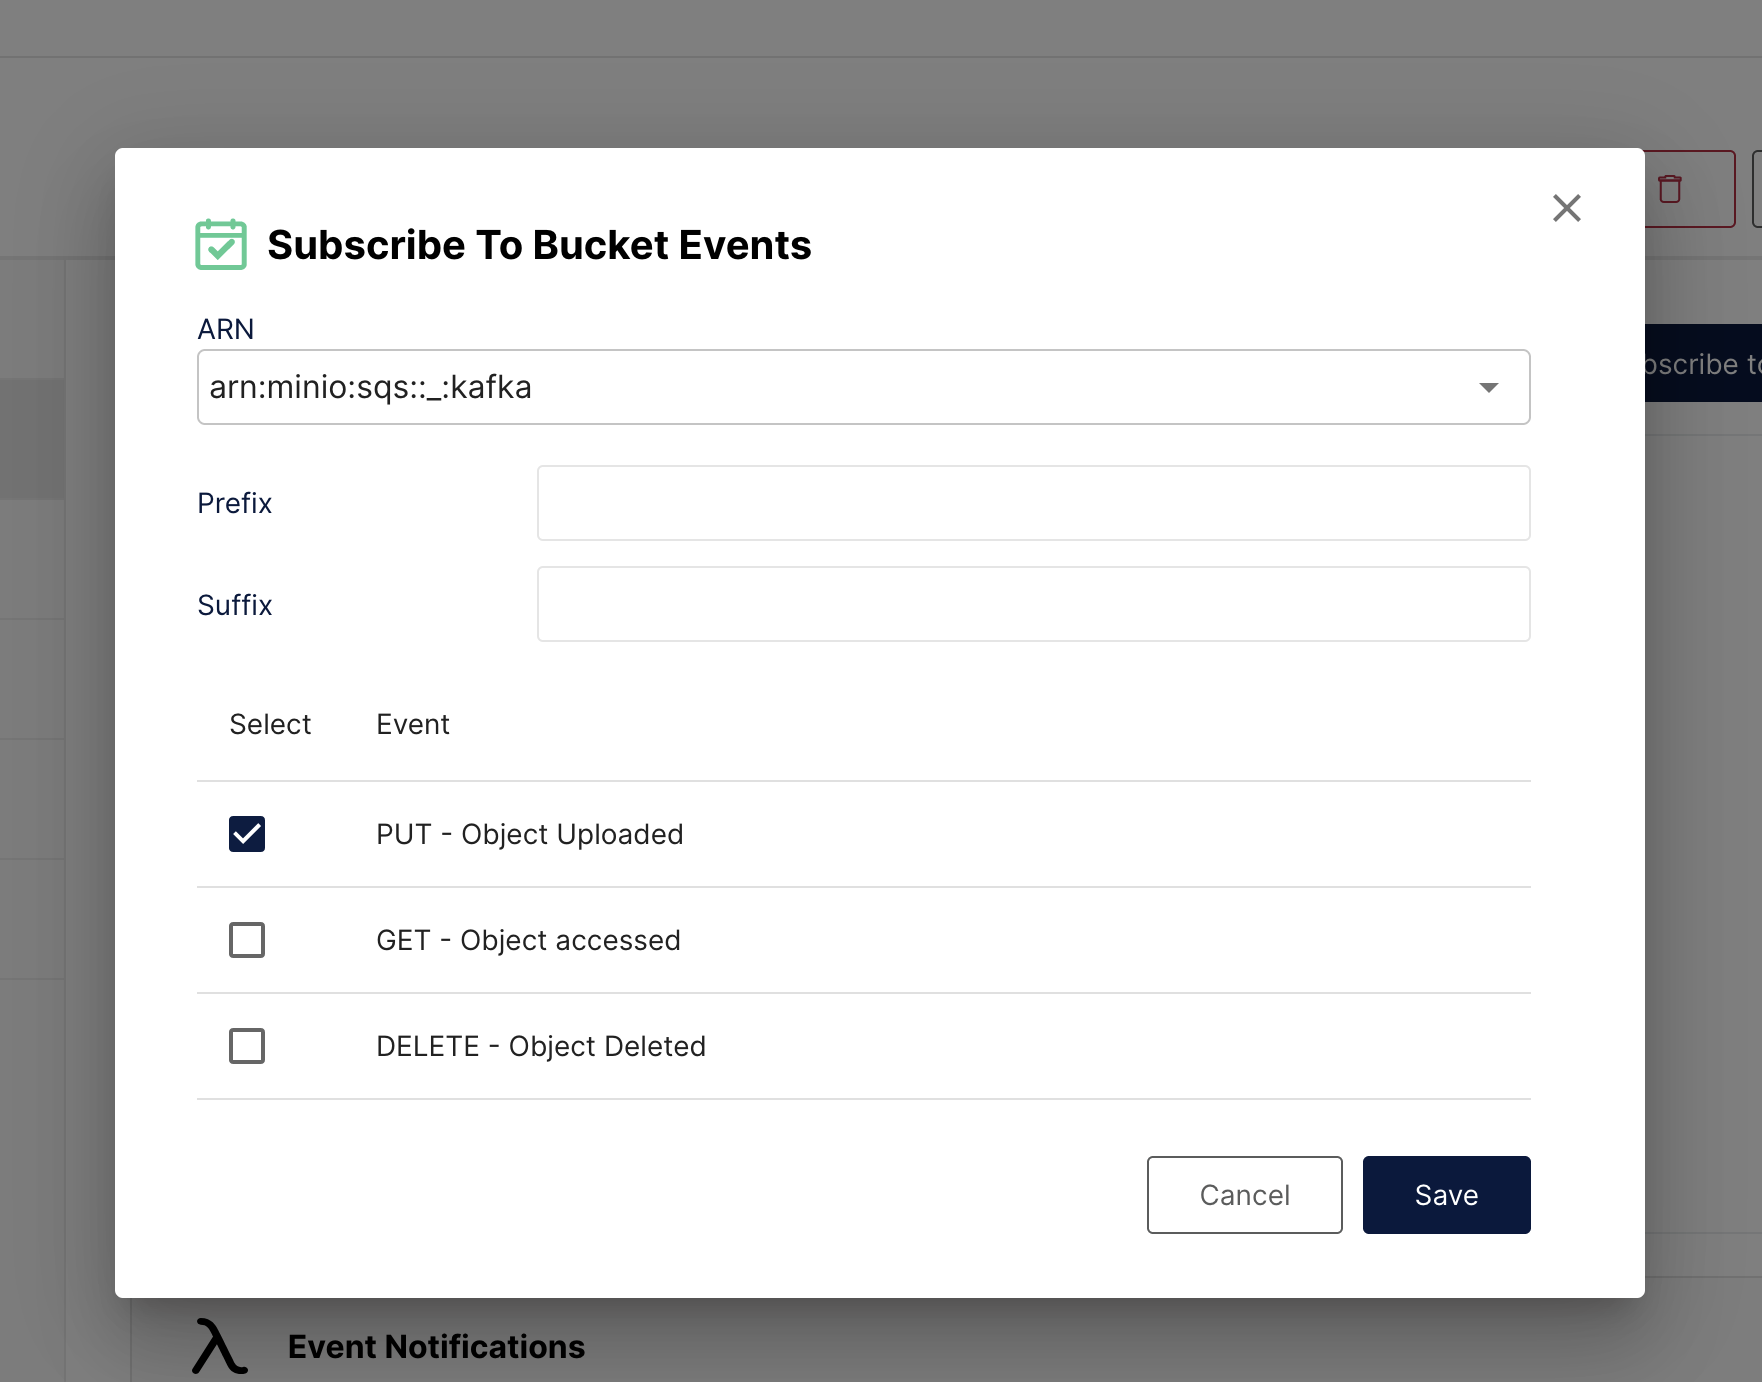
\includegraphics[scale=0.31]{images/minio-bucket-event.png}
  \caption{Registering Bucket to Send Events to Kafka}
  \label{appendix:minio-bucket-event}
\end{figure}

\lstinputlisting[basicstyle=\tiny, language=SQL, caption={Aegis Scan
  Log}, label=appendix:aegis-logs]{assets/aegis-logs.txt}

\begin{figure}[H]
  \centering 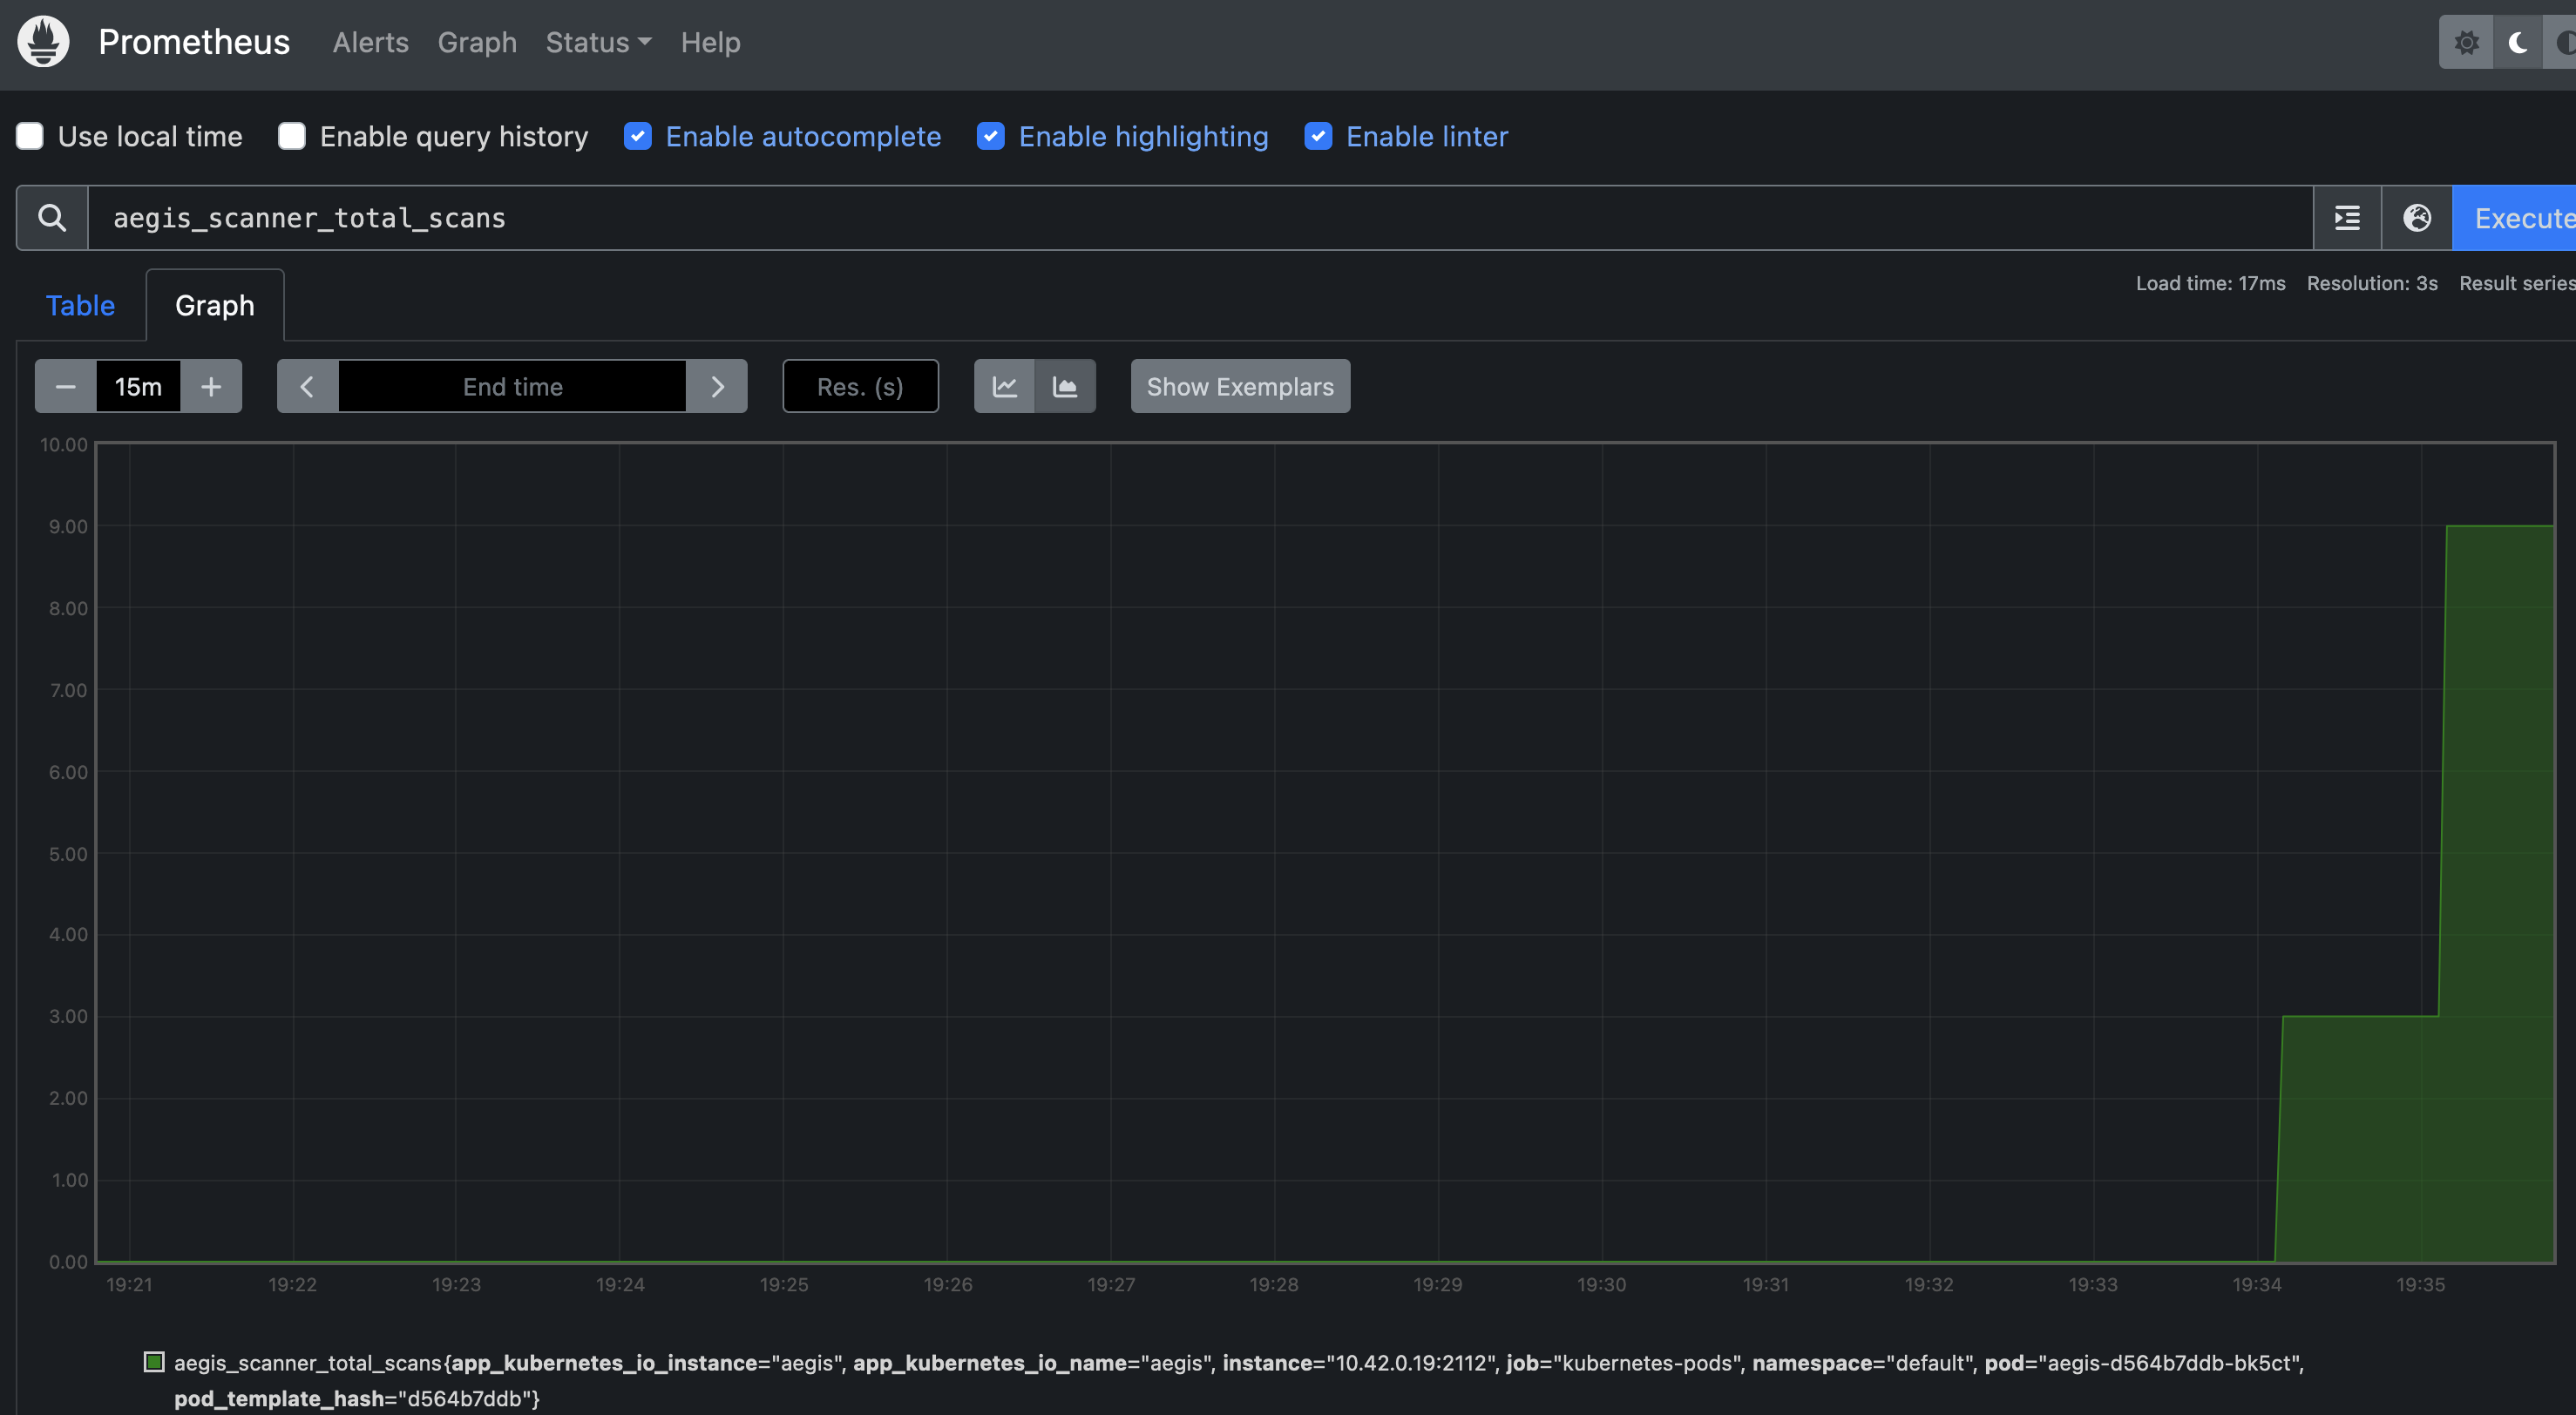
\includegraphics[scale=0.31]{images/prometheus-metrics.png}
  \caption{Exposed Prometheus Metrics}
  \label{appendix:prometheus-metrics}
\end{figure}

\lstinputlisting[basicstyle=\tiny, language=SQL, caption={Example Audit
  Log}, label=appendix:audit-log]{assets/audit-logs.txt}

\bigskip \lstinputlisting[caption={Output of Unit Tests},
label=appendix:go-tests]{assets/test-logs.txt}

\lstinputlisting[basicstyle=\tiny, caption={Output of kubectl get all},
label=appendix:kube-get-all]{assets/kube-get-all.txt}

\lstinputlisting[basicstyle=\tiny, caption={Shutdown Logs of Aegis},
label=appendix:shutdown-logs]{assets/shutdown-logs.txt}
\bigskip

\bibliographystyle{cardiff} \bibliography{references}

\end{document}
